\chapter*{Additional Problems}
\label{chap:additional_problems}
\addcontentsline{toc}{chapter}{Additional Problems}
\markboth{ADDITIONAL PROBLEMS}{ADDITIONAL PROBLEMS}


\begin{aproblem}{Repulsive and attractive tape.}  
  Take some magic Scotch tape and tear off a piece about 6 inches
  long.  Attach it to the edge of a desk or table so that it hangs
  down.  Then get another piece and stick the new (top) piece to the
  non-sticky side of the first (bottom) piece. Then quickly pull them
  apart and hang both of them from edge of the table.  Label the strip
  that had been initially on the top ``T'' and label the other one
  ``B.''
  \begin{enumerate} 
  \item Next hold them so that the ends can come near each other.  Do
    they attract?  Repel?  Neither?  Try to write down a brief
    explanation.
  \item Take two more pieces of tape and repeat the above so that you
    have two T's and two B's.  Which pairs attract and which repel?
    Why?
  \end{enumerate}
\end{aproblem}

\begin{aproblem}{Repulsive balloons.}  
  Blow up two balloons (not quite as full as possible) and tie them so
  they don't leak.  Take a piece of string and attach (tie or tape) a
  balloon to each end, then hold the string in the middle and let the
  balloons at each end hang down.
  \begin{enumerate}
  \item Now charge up the balloons by rubbing them against a fuzzy
    sweater or whatever you're wearing.  Be sure to turn the balloon
    so that all parts get charged.  Holding the string in the middle
    (and keeping your body parts away from the balloons!), what do you
    observe about the way the balloons hang?  Make a sketch.  Then
    make a force diagram for one of the balloons, showing all of the
    forces acting on the balloon (tension, electric and gravitational)
    and their relative magnitudes.  \textbf{Note:} Since the
    balloons are in equilibrium, your force vectors should add up to
    zero.  Make sure that they are drawn to reflect this.
  \item Now, carefully grab one balloon and push it slowly toward the
    other.  Make sure that the balloons stay at the same height, so
    that a line through their centers remains roughly horizontal.
    What happens to the distance between the balloons as the string on
    the non-held balloon makes bigger and bigger angles with the
    vertical?  When you have moved the held balloon enough so that the
    distance between the balloons is clearly different from that in
    part (a), make a force diagram for the non-held balloon, showing
    all the forces and their relative magnitudes.  (The sizes of the
    arrows should also reflect any changes in the forces with respect
    to part (a).)  \textbf{Comments: } Again, the balloon is in
    equilibrium, so the force vectors should add up to zero.  But
    since your tension force is closer to horizontal now, what has to
    happen to its magnitude to keep the net force in the $y$-direction
    zero?  What has to happen to the electric force to keep the net
    force in the $x$-direction zero?  Make sure that your diagram is
    consistent with your observation about the distance between the
    balloons.
  \end{enumerate}
\end{aproblem}


\begin{aproblem}{Attractive balloons.}  
  The figure shows two balloons, one with a positive charge $q$ and
  one with a negative charge $q$, each hung from the ceiling by a
  thread, as shown.  The system is in equilibrium, and each thread
  makes an angle $\theta$ with respect to the vertical. Show that the
  charge $q$ on the balloons is given by $q =
  x\sqrt{\frac{mg\tan\theta}{k}}$.
  \label{prob:balloons}

  \begin{figure}[h]
    \begin{center}
      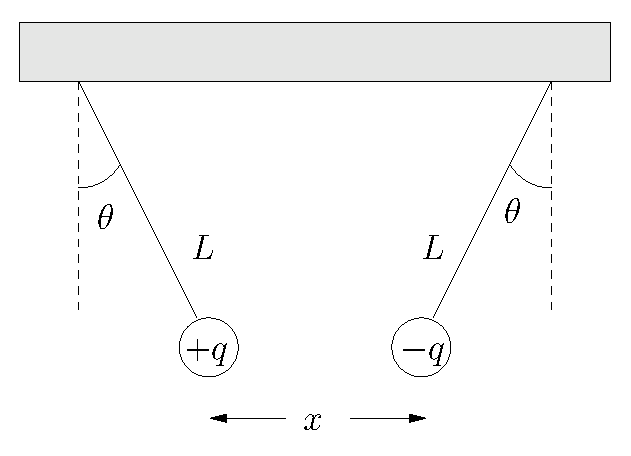
\includegraphics[width=5cm]{additional_problems/ballooncalc}
      \caption{Problem A\ref{prob:balloons}}
    \end{center}
  \end{figure}
\end{aproblem}


\begin{aproblem}{Electric field simulations.}  
  Do Problem 1 on Electric Fields, accessible from the Lecture 1
  calendar page.
\end{aproblem}


\begin{aproblem}{More E-Field Simulations.} 
  Do Problem 2 on Electric Fields, accessible from the Lecture 1
  calendar page.
\end{aproblem}

\begin{aproblem}{Addition of electric fields.} 
  Two charges, each $+5~\mu$C, are on the $y$-axis, one at the origin
  and the other at $y=6\units{m}$.  Find the electric field on the
  $y$-axis at (a) $y=-3\units{m}$, (b) $y = +3\units{m}$, and (c) $y =
  +9\units{m}$.
  \label{prob:addEfields}
\end{aproblem}

\newpage

\begin{aproblem}{Determining $\vec{E}$ using integrals --- semi-infinite rod.} 
  Point {\bf P} is located a distance $a$ from the bottom of a
  semi-infinite rod with uniform linear charge density $\lambda$.
    \begin{enumerate}
    \item Calculate the $x$-component of the electric field at point
      {\bf P}; you should set up and work through the integral.
    \item Calculate the $y$-component of the electric field at point
      {\bf P}; you should set up and work through the integral.
      (Somewhat surprisingly the $x$ and $y$-components have the same
      magnitude.)
    \end{enumerate}
    \label{prob:integ1}

    \begin{figure}[h]
      \begin{center}
        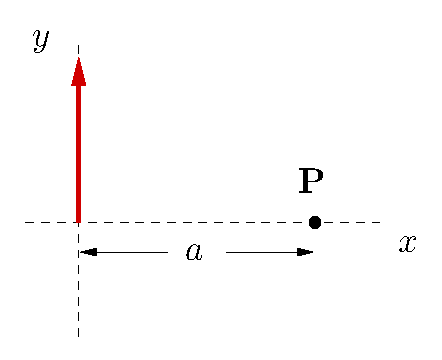
\includegraphics[width=5cm]{additional_problems/integ1}
        \caption{Problem A\ref{prob:integ1}}
      \end{center}
    \end{figure}
\end{aproblem}


\begin{aproblem}{Determining $\vec{E}$ using integrals --- arc.}  
  The figure shows a quarter of a ring with radius $R$ in the $x$-$y$
  plane with a total charge $q$, which is distributed uniformly over
  the quarter-ring. Working through the appropriate integral,
  determine the electric field at the origin (point {\bf P}).
  \label{prob:arc1}

  \begin{figure}[h]
    \begin{center}
      \scalebox{0.7}{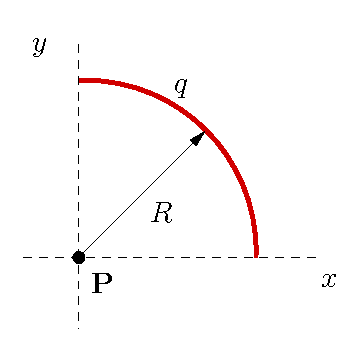
\includegraphics{additional_problems/arc1}}
      \caption{Problem A\ref{prob:arc1}}
    \end{center}
  \end{figure}
\end{aproblem}

\newpage

\begin{aproblem}{Computer monitors.} 
  In a computer monitor (the old-fashioned tube-type monitor, not the
  flat panel ones), electrons are fired from the back toward the
  screen.  Assume that the electrons start from rest and are
  accelerated through a potential difference of 50,000 V.
   \begin{enumerate}
   \item What is the energy of the electrons when they hit the screen
     in electron volts?
   \item in Joules?  
   \item What is the speed of impact of the electrons with the screen
     of the monitor?  (You can neglect relativistic effects here,
     although you should note that the speeds aren't {\it that} much
     below the speed of light.)
   \end{enumerate}
   \label{prob:ComputerMonitors}
\end{aproblem}

\begin{aproblem}{Directions of electric fields from continuous sources.}
  The figure shows half of a ring in the $x$-$y$ plane with a varying
  charge density $\lambda$ which depends on the angle $\theta$ from
  the $+x$-axis.
  \begin{enumerate}
  \item Determine the {\bf direction} of the electric field at the
    origin (point {\bf P}) if $\lambda = \lambda_0 \sin{\theta}$.
  \item Determine the {\bf direction} of the electric field at the
    origin (point {\bf P}) if $\lambda = \lambda_0 \cos{\theta}$.
  \end{enumerate}
  \label{prob:arc2}
  \begin{figure}[h]
    \begin{center}
      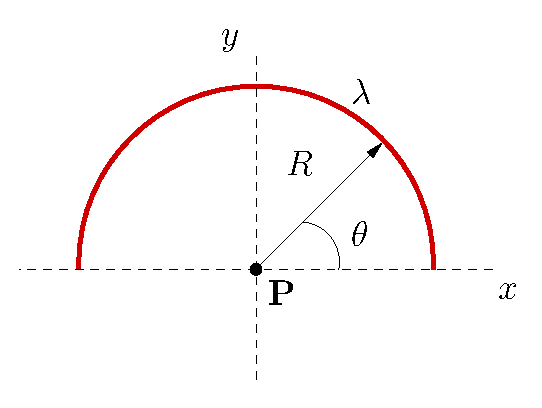
\includegraphics[width=5cm]{additional_problems/arc2}
      \caption{Problem A\ref{prob:arc2}}
    \end{center}
  \end{figure}
\end{aproblem}

\newpage

\begin{aproblem}{Potential and electric field.} 
  The sketch shows three large parallel plate conductors held at the
  potentials shown. (Assume that the plates are infinitely large.)
  Find the direction and magnitude of the uniform electric field in
  each of the two interior regions. \label{prob:plates}
  \begin{figure}[h]
    \begin{center}
      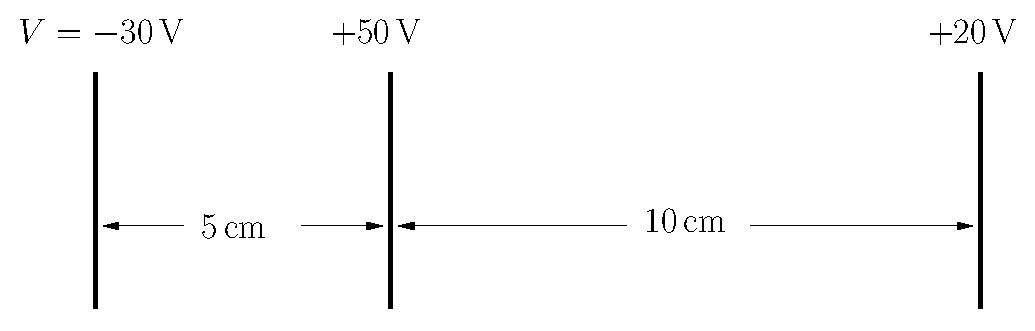
\includegraphics[width=10cm]{additional_problems/plates}
      \caption{Problem A\ref{prob:plates}}
    \end{center}
  \end{figure}
\end{aproblem}


\begin{aproblem}{Resistance and Dimmer Switches.}
  \begin{enumerate}
  \item Make a circuit with two batteries and a light bulb, all in
    series, and note the brightness.  Now add a full length of one of
    your nichrome wires (bare silvery wire) to your circuit between
    the positive side of your batteries and the bulb.  What happens to
    the brightness of the bulb?  Explain briefly.
  \item Repeat with the other equal length piece of nichrome wire.
    Which wire has a larger resistance? % A larger resistivity?
    Explain how you know.  Examine the two wires carefully.  Do you
    note any difference?
  \item Now use just the higher resistance wire in the circuit.
    Carefully unclip the lead on the wire nearest the battery, and
    touch it onto the wire at various places.  How is the bulb's
    brightness affected?  This is basically how a dimmer switch works!
  \end{enumerate}
  \label{prob:dimmer}
\end{aproblem}

\begin{aproblem}{Flashlight circuit}
  Make a circuit with two batteries and two bulbs, all in series.
  \begin{enumerate}
  \item Now replace one of the bulb holders in the circuit with the
    higher resistance nichrome wire, and slide the alligator lead from
    the batteries along the wire (see Prob.~A\ref{prob:dimmer}) until
    the remaining bulb is about as bright as before with the two
    bulbs. This means the resistance of that length of nichrome is the
    same as a bulb. Measure this length.
  \item The wire has a diameter of $0.25\units{mm}$, and the
    resistivity of nichrome is $\rho = 1.0 \times
    10^{-6}\units{$\Omega\cdot$m}$.  Calculate the resistance of the
    length of wire, and therefore of the bulb.  {\bf Continued}$\rightarrow$
  \item From the battery voltage and the resistance that you just
    determined for one bulb, determine the current through the
    original circuit with two bulbs and two batteries.
  \end{enumerate}
\end{aproblem}


\begin{aproblem}{Fun with magnets.}
  Take two cylindrical magnets and let them come together (N of one
  and S of other) around the end of a piece of thread (see
  Fig.~\ref{fig:compass}). You'll end up with what is effectively one
  long magnet (from the two in combination) with a string coming up
  from in between the two (now connected) magnets.  Hold the other end
  of the string and let the magnet dangle.  Now gently twist the
  string from the top. Is there a preferred orientation for the
  magnet? What is this orientation? Explain briefly.
  \label{prob:compass}

  \begin{figure}[h]
    \begin{center}
      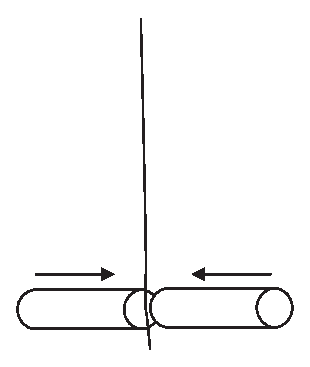
\includegraphics[width=4cm]{additional_problems/compass}
      \caption{Problem A\ref{prob:compass}} \label{fig:compass}
    \end{center}
  \end{figure}
\end{aproblem}


\begin{aproblem}{Mapping the field of a permanent magnet.}
  \begin{enumerate}
  \item Draw a sketch of a cylindrical magnet including the direction
    of the magnetic field in the surrounding region. Mark the
    direction of the magnetic field with little arrows at various
    locations around the magnet.
  \item Now put your cylindrical magnet down on a flat surface and
    keep it from rolling.  Next place your compass in various
    positions around the magnet and draw a sketch of what you observe.
    Your sketch should show a long rectangle (the magnet) surrounded
    by circles (the compass in various locations) with an arrow on
    each circle showing the direction that the red part of the compass
    needle pointed there.  How did your measurements compare to your
    prediction?
  \end{enumerate}
\end{aproblem}

\newpage

\begin{aproblem}{Destroying your TV or computer monitor.}
  (Optional) BE CAREFUL with this one. A strong permanent magnet can
  magnetize parts of your monitor. This causes distortion of the
  images in both shape and color. Most monitors automatically can get
  rid of these extra fields using something called a ``de-gausser'',
  but the de-gausser doesn't usually activate except when the monitor
  is turned on (and is cold), so it might not fix the damage for a
  while, assuming the de-gausser is working.  Thus the caution. Most
  monitors receive no permanent damage, but you never know, so don't
  go wrecking someone else's stuff.

  Bring one of your magnets close to a CRT, like a computer monitor or
  TV. Move the magnet around the front and along the top and
  sides. Write down your observations.  Why does this happen?  What is
  a CRT anyway?
\end{aproblem}


\begin{aproblem}{Magnetic force on a moving particle.}  
  The figure shows a charged particle (with charge
  $-5.0\units{$\mu$C}$) moving with a speed $1.3 \times
  10^5\units{m/s}$ in a vertically-directed magnetic field with
  magnitude $0.8\units{T}$.  The particle is moving at an angle
  $30^{\circ}$ with respect to the horizontal.  Calculate the
  magnitude of the magnetic force on this particle, and state the {\bf
    direction} of the force. \label{prob:magforce}

  \begin{figure}[h]
    \begin{center}
      \scalebox{0.7}{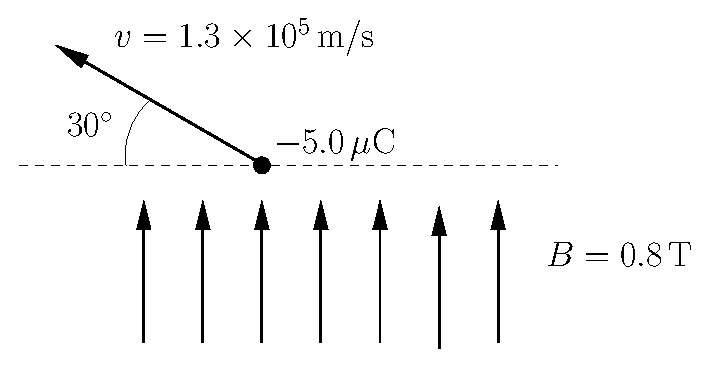
\includegraphics{additional_problems/magforce}}
    \end{center}
    \caption{Problem A\ref{prob:magforce}}
  \end{figure}
\end{aproblem}

\newpage

\begin{aproblem}{Rail guns.}  
  A very simple application of magnetic forces can be used to make a
  nifty device called a ``rail gun.'' These have been proposed as
  devices that could be used to send back to earth (or the moon) raw
  materials mined from an asteroid.  The idea is shown in the figure
  below.  A bar of mass $m$ can slide on two parallel rails separated
  by a distance $H$, and the whole apparatus is in a uniform magnetic
  field with magnitude $B$ pointing into the plane of the paper.  The
  rails are hooked up to a current source, and a current $I$ passes
  through the rails and through the bar, which experiences a force
  that accelerates it down a track of length $D$.  A bucket can be put
  on the bar, and anything in the bucket gets thrown off when the bar
  reaches the end of the rail.

  Given the information above, determine the speed of the bar just
  before it reaches the end of the rails.  (Hint: Think work.)
  \label{prob:railgun}
  \begin{figure}[h]
    \begin{center}
      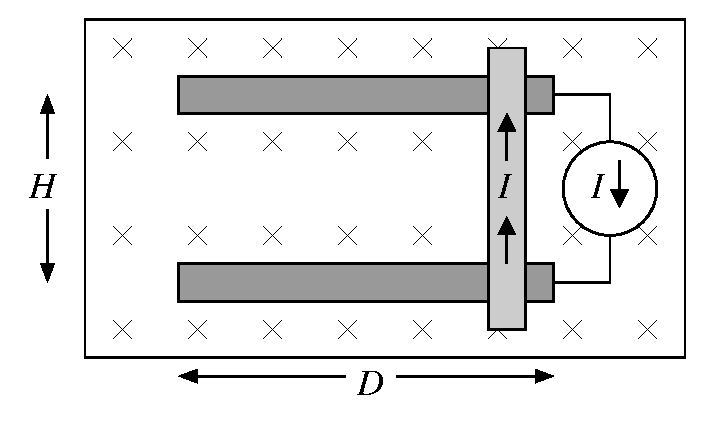
\includegraphics[width=6cm]{additional_problems/railgun}
      \caption{Problem A\ref{prob:railgun}}
    \end{center}
  \end{figure}
\end{aproblem}

\begin{aproblem}{Canceling the Earth's magnetic field.}  
  A 100-turn circular coil with radius $30\units{cm}$ is to produce a
  field at its center that will just cancel the earth's magnetic field
  at the equator, which is $7.0 \times 10^{-5}\units{T}$ directed
  north (horizontal). Find the current in the loop and make a sketch
  that shows the orientation of the loop and the current.
\end{aproblem}


\begin{aproblem}{Why aren't there magnetic fields all around your
house?}
  \begin{enumerate}
  \item The wire to a 100 Watt lamp carries about 1 amp of current to
    light the lamp. Calculate the magnetic field $5\units{mm}$ from a
    wire carrying a steady current of 1 amp.  Compare this to the
    Earth's field of approximately $7 \times 10^{-5}\units{T}$.
  \item Put your compass near various wires in your room leading to
    electrical appliances and lights.  Describe the compass
    deflections.  Why don't you see much?  (Hint: The power cords
    aren't just one wire but are a pair that carry the current both
    {\bf to} and {\bf back from} the appliance/light.)
    \label{prob:PowerCords}
  \end{enumerate}
\end{aproblem}

\begin{aproblem}{An electromagnet.}  
  Take your large and small nail and put them on a table top. Clip one
  end of an alligator lead to a battery (or two in series). Clip
  another to the opposite side of the battery. Wrap the piece of red
  insulated wire many, many times around the larger nail. Hold the
  wrapped nail in one hand and using the other, hook the leads from
  the batteries onto the ends of the wrapped wire to complete the
  circuit.  You're making an electromagnet!

  Try to pick up the small nail with the point of the large nail.
  Once it is off the table, disconnect the leads and see what happens.
  On your paper, explain briefly why the nail becomes a magnet.
\end{aproblem}

\begin{aproblem}{Solenoid.}  
  A solenoid with 2000 turns is $1.3\units{m}$ long, has a radius
  $2.5\units{cm}$ and carries a current of $3.0\units{A}$.  What is
  the approximate magnitude of the magnetic field on the axis near the
  center of the solenoid?
  \label{prob:solenoid}
\end{aproblem}


\begin{aproblem}{Electrical generation.}  
  Commercial electricity generation uses big strong magnets,
  multi-turn coils, and rapid relative motion.  Suppose you could move
  a large $1.0\units{T}$ magnet over the face of a $10\units{cm}$
  diameter 200-turn coil.  What time interval between maximum flux and
  no flux would you need to produce an average emf of $120\units{V}$?
  \label{prob:ElecGen}
\end{aproblem}


\begin{aproblem}{Faraday with derivatives.} 
  A ring with radius $r$ and resistance $R$ lies in the $x$-$y$ plane.
  The ring is located in a spatially uniform, but time-dependent
  magnetic field $\vec{B} = B_0(2-t+3t^2)\, \widehat{k}$.  Calculate
  the magnitude of the electrical current $I(t)$ in the ring as a
  function of time.
  \label{prob:faraday}
\end{aproblem}

\begin{aproblem}{Eddy damping and brakes.} 
  Describe how eddy currents could be used to make brakes for a train
  or a car that don't require any friction.
\end{aproblem}

\begin{aproblem}{The Electromagnetic Spectrum.}  
  Consider the different types of electromagnetic waves: radio waves,
  microwaves, infrared, visible light, ultraviolet light, x-rays and
  gamma rays.  Why do you think there are different names for these
  different kinds of electromagnetic waves?  Is there a meaningful
  distinction?  What are the differences between, say, gamma rays and
  infrared waves?
\end{aproblem}


\begin{aproblem}{Electromagnetic waves and you}.  
  Think about your life, your experiences and things which you may
  {\it not} have experienced but which clearly affect your life. There
  are numerous situations in which electromagnetic waves play a
  significant role in affecting your life.  List {\bf at least} four
  distinct and unique examples.  These list might include things like
  examples of modern technology which rely on electromagnetic waves,
  as well as important electromagnetic wave phenomena which occur in
  the natural world.
\end{aproblem}


\begin{aproblem}{Falling loops.}  
  A long rectangular wire loop with mass $m$ and resistance $R$ is
  falling out of a region with a magnetic field with magnitude $B_0$
  that is pointing out of the plane of the paper.  The rectangle has a
  width $w$ and a length that is so large that part of the loop is
  inside the region with the magnetic field and part is outside that
  region;
  \begin{enumerate}
  \item Determine the current in the wire when the rectangle is
    falling from the magnetic field with a speed $v$.
  \item When dropped from rest the speed of the loop increases from
    $0$ up to the terminal velocity, and then remains constant at this
    terminal velocity.  Determine the terminal velocity for the
    falling loop.  (Assume that the terminal velocity is reached
    before the top of the loop leaves the magnetic field.)
  \end{enumerate}

  \begin{figure}[h]
    \begin{center}
      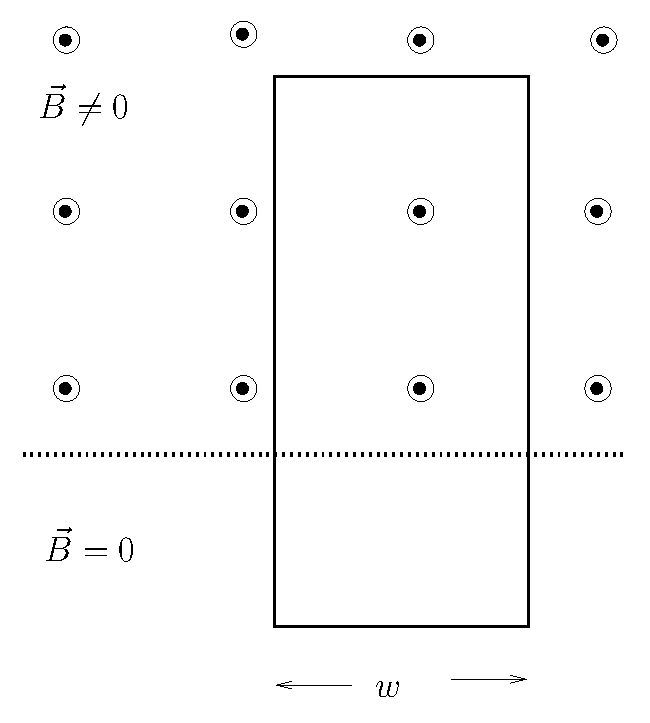
\includegraphics[width=5cm]{additional_problems/bu_em_falling-loop}
      \caption{Problem A\ref{prob:bu_em_falling-loop}}
    \end{center}
  \end{figure}
  \label{prob:bu_em_falling-loop}
\end{aproblem}


\begin{aproblem}{Fetal heartbeat monitors.}  
  The {\it Babycom}$^{\rm TM}$ {\it Home Doppler Fetal Heartbeat
    Monitor} uses ultrasonic waves with frequency $2.5\units{MHz}$,
  and can measure Doppler shifts as low as $100\units{Hz}$.  Calculate
  the approximate speed of the fetal movements (blood flow) that
  account for these $100\units{Hz}$ frequency shifts.  (The speed of
  sound in air is $340\units{m/s}$, and the speed of sound in soft
  tissue --- and water --- is about $1500\units{m/s}$.)
\end{aproblem}


\begin{aproblem}{Electromagnetic waves.} 
  Consider an EM wave with electric field $\vec{E} = (6.6 \times
  10^4\units{N/C})\cos(1.2\pi x - 3.6 \times 10^8 \pi t)\,
  \hat{\jmath}$ with $x$ in meters and $t$ in seconds.  Find the
  expression for the corresponding magnetic field.
\end{aproblem}

\newpage

\begin{aproblem}{Re-radiated Light Waves.}  
  Consider a beam of light propagating along the $y$-axis.  It is
  polarized along the $z$-axis as it enters a diffuse vapor cloud.
  \begin{enumerate}
  \item Along which axis does the electric field of the light wave
    oscillate ($\pm x$, $\pm y$, or $\pm z$)?  How do you know?
  \item Along which axis does the {\it magnetic} field of the light
    wave oscillate ($\pm x$, $\pm y$, or $\pm z$)?  How do you know?
  \item The wave strikes some electrons in the vapor cloud, and they
    start oscillating.  Along which axis do the electrons oscillate
    ($\pm x$, $\pm y$, or $\pm z$)?  How do you know?
  \item These oscillating electrons generate a new re-radiated light
    wave. Along which axis does the electric field of the re-radiated
    wave oscillate ($\pm x$, $\pm y$, or $\pm z$)?  How do you know?
  \item The re-radiated light wave cannot propagate in all directions.
    Along which axis (axes) can the new wave propagate ($\pm x$, $\pm
    y$, or $\pm z$)?
  \item For each answer to part (e), give the axis along which the
    {\it magnetic} field of the re-radiated wave oscillates ($\pm x$,
    $\pm y$, or $\pm z$).
  \end{enumerate}
  \label{prob:reradiation}
\end{aproblem}


\begin{aproblem}{Traveling Waves on a Magic Spring.} 
  Take your Magic Spring and attach one end to a door knob, bed post
  or a friend.  Hold the other end and walk away so the spring is
  stretched to about 6 feet.  Grab a few of the coils and pull them
  toward you and release so that a longitudinal compression wave
  travels along the spring, bounces off the other end, and goes back
  and forth.  See how far the pulse goes in five seconds (\# of round
  trips times round-trip distance) and estimate the wave speed.
  Repeat by pulling the coils sideways to get a transverse wave, and
  find its wave speed.  Are they different?  Compare to the speeds
  found in Question A\ref{a:standingwave}. \label{a:travwave}
\end{aproblem}


\begin{aproblem}{Standing Waves on a Magic Spring.}  
  Find a friend to help you time and count Magic Spring standing wave
  oscillations.
  \begin{enumerate}
  \item Hold the spring with one end in each hand and generate
    standing waves as demonstrated in lecture.  Get at least the
    fundamental and the next two higher harmonics.  (Prize if you can
    demonstrate the $n=5$ mode or higher!)  Notice how the frequency
    you need to use changes for as the mode number increases.
  \item For quantitative analysis, set up the spring just as you had
    it when you measured pulse speeds in Question A\ref{a:travwave}.
    Set up the lowest frequency standing wave by shaking one end of
    the spring and count ten full oscillations while your friend
    measures the time for these ten oscillations.  Determine the
    period, frequency, and wavelength for this mode.  Repeat your
    measurements for the $n=2$ and $n=3$ modes, making sure that you
    keep the length of the spring (the distance between your ``shaking
    hand'' and the fixed end) approximately the same for all of your
    measurements.
  \item What is the ratio of the frequency of the $n = 2$ mode to the
    fundamental frequency?  What is the ratio of the frequency of $n =
    3$ mode to the fundamental?  Is this what you expect?
  \item Use the wavelength and corresponding frequency for each mode
    to determine a wave speed.  Compare these to the speed of
    transverse waves measured in Question A\ref{a:travwave}.
  \end{enumerate}
  \label{a:standingwave}
\end{aproblem}


\begin{aproblem}{A musical octave.}  
  Use your slide whistle for this one.
  \begin{enumerate}
  \item Extend the slide all the way out.  Blow softly on the whistle
    and note the pitch.  Now push the slide in as you continue to
    blow.  What do you hear?  Explain {\it why} you hear the changes
    in the pitch that you hear when the slide is pushed inward.
  \item Extend the slide all the way out again.  Again, blow softly on
    the whistle and note the pitch.  Now continue to play the whistle
    as you push the slide inward, and stop when you reach a note that
    is an octave above what you started with. (This may take many
    tries to match.)  What determines how far the slide should be
    pushed in to increase the pitch by one octave?  Try to see if you
    can make a simple (approximate) measurement to verify your theory.
  \end{enumerate}
\end{aproblem}


\begin{aproblem}{Annoying your roommate.} 
  Here is another opportunity to play with your slide whistle.
  \begin{enumerate}
  \item Play the slide whistle softly with the slide mostly or all the
    way out.  Make a sketch of the standing wave in the air column
    associated with this note.
  \item Now blow harder on the slide whistle until the pitch changes.
    How is the frequency of this new (and most assuredly
    less-pleasant-sounding) note related to the one from part (a)?
    Draw a sketch of the standing wave to support your answer.
  \item Now plug your ears and blow even harder.  You should be able
    to get the pitch to jump again (and to attract any stray dogs that
    are in the neighborhood, along with a few irate hall-mates). How
    is the frequency of {\it this} note related to the one from part
    (a)?  Draw a sketch of the standing wave to support your answer.
  \end{enumerate}
\end{aproblem}

\newpage

\begin{aproblem}{Organ pipes.}  
  Consider a $10\units{m}$ organ pipe, open at both ends.
  \begin{enumerate}
  \item Sketch the standing wave pattern for the three longest
    wavelength modes.
  \item From each sketch, determine the wavenumber $k$ and the
    wavelength $\lambda$.
  \item Given your answers for (a) and (b), and given the speed of
    sound in air ($340\units{m/s}$), determine the frequency of each
    mode.
  \end{enumerate}
  \label{prob:OrganPipes}
\end{aproblem}


\begin{aproblem}{Stringed instruments.} 
  The lowest note that can be played on a bass fiddle is E1 (frequency
  41.2 Hz) on a string of length $1.2\units{m}$ (secured at both
  ends).
  \begin{enumerate}
  \item Sketch the standing wave pattern for the three longest
    wavelength modes.
  \item From each sketch, determine the wavenumber $k$ and the
    wavelength $\lambda$.
  \item Determine the wave speed for this string.
  \end{enumerate}
\end{aproblem}

\begin{aproblem}{Beats.}  
  Find someone else who is taking PHYS 212. One of you should blow
  (softly) your slide whistle with the slide somewhere in the
  middle. Hold the note while the other person blows his/her whistle
  and slowly adjusts his/her slide around the position of your slide.
  Listen for the beats and comment on how they change as the frequency
  of the second whistle is varied.
\end{aproblem}


\begin{aproblem}{Polarized light.}  
  Take your polarized disks and look at the following things and
  comment on what you observe:
  \begin{enumerate}
  \item Go outside on a sunny day when the sun is low in the sky,
    preferably early or late in the day and look straight up at the
    sky, looking through one of the Polaroid disks.  Then turn the
    disk.  What do you observe?  What does this tell you about light
    scattered from the sky?
  \item Look at various different LCDs (liquid-crystal displays): your
    calculator, a laptop or flat-screen monitor, a gas station pump
    readout, etc.  Rotate the Polaroid disk and comment on what you
    observe.  What does this tell you about liquid-crystal displays?
  \item How could you determine definitively if some sunglasses that
    you were buying at Wal-Mart$^{TM}$ were polarized?  (Don't trust
    the labels: my wife once bought ``polarized'' sunglasses that
    turned out to be fakes.)
  \end{enumerate}
\end{aproblem}

\newpage

\begin{aproblem}{Soap films and bubbles.} 
  \begin{enumerate} 
  \item Here's one to try in the shower! Get your hands very wet and
    soapy. Then slowly slide your forefinger along your thumb
    stretching a soap film bigger and bigger.  You can catch it on
    your other hand as demoed in lecture to make a big thin film.  In
    fact, if your hands are wet, you can catch soap bubbles without
    popping them. (This is a great thing to do on a day just after it
    has rained --- blow a bunch of soap bubbles on the wet pavement.
    They won't pop.)

    If you are not good at this, try using bubbles from the soap
    bubble bottle in your kit.  Blow a big bubble, catch it on the
    wand, and hold it while it thins out.

    Now with the light behind you, look at the reflections off the
    film. You should see some really cool patterns of colors!  Try to
    sketch the patterns (later) and show where each color is.  In a
    few sentences, try to explain what you see in terms of thin films
    that you studied in class.

  \item (Optional if weather cooperates.)  After it has rained, look
    at the pavement in the street or parking lots where cars are or
    have been.  You might see a blotch of color.  This usually
    indicates that a drop of oil has fallen on the ground.  (A good
    place to look for these splotches is underneath cars driven by
    Bucknell faculty.) If you see one of these colorful oil spots, try
    stepping on it or brushing your foot over it.  Comment on what you
    see and try to explain what you see in terms of the thin films
    that you studied in class.
  \end{enumerate}
\end{aproblem}


\begin{aproblem}{Fiber optics toy.} 
  Load up your fiber optics flashlight toy (Galaxy Wand) with the two
  little batteries (this may have already been done for you). Turn it
  on and notice how the cool colors of light come out the ends of the
  fibers but not out the sides.  Take one of the fibers and bend it
  until it kinks. (If it breaks, try again.)  Some of the light in
  that fiber will escape.  Why does it escape?  Why doesn't it escape
  if you make smooth curves in the fiber rather than a kink?
\end{aproblem}


\begin{aproblem}{Thin film interference.} 
  Assume that light with a wavelength $\lambda_0$ in air falls on a
  thin film composed mostly of water (index of refraction $n_w$) and
  with a thickness $t$.  Assume that the water is on top of a mirror
  which inverts the EM wave when it reflects it.
  \begin{enumerate}
  \item What is the wavelength of the light inside the film (in terms
    of $\lambda_0$ and $n_w$)?
  \item What is the path length difference between the light reflected
    off the front of the film and that which goes through the film,
    reflects off the mirror, and {\it then} comes back through the
    film and out the front?
  \item Are either (or both) of the two beams of reflected light
    inverted due to the reflection?
  \item What is the phase difference between the two reflected beams?
    (Hint: use the wavelength of the light {\it inside} the water
    film.
  \item If $n_w = 1.33$ and the film has a thickness $t =
    300\units{nm}$, what is the largest wavelength of light (when in
    air) for completely destructive interference?  For completely
    constructive interference?
  \end{enumerate}
\end{aproblem}


\begin{aproblem}{Son of thin film interference.} 
  Assume that light with a wavelength $\lambda_0$ falls on a thin film
  composed mostly of water (index of refraction $n_w$) and with a
  thickness $t$. Assume that the film is surrounded by air on both
  sides.

  If $n_w = 1.33$ and the film has a thickness $t = 300\units{nm}$,
  what is the longest wavelength of light (when in air) for completely
  destructive interference in the reflected light?  For completely
  constructive interference?
\end{aproblem}


\begin{aproblem}{Interference in music.}  
  Sitting at your desk, you are listening to music from your stereo.
  Your right ear is $2.2\units{m}$ from one speaker and $2.6\units{m}$
  from the other.  Nostalgic for your formative childhood years, you
  are listening to a {\it Barney's Greatest Hits} CD, and there is a
  particular solo by Barney in which the frequency of his tune ranges
  up to $1800\units{Hz}$.  Ignoring reflections, determine the two
  smallest frequencies at which there will be destructive interference
  of the sound at your right ear; i.e., where the sound will be
  weakest.
\end{aproblem}


\begin{aproblem}{DVDs.}  
  If you shine laser light with wavelength $650\units{nm}$ at normal
  incidence onto the surface of DVD, you'll find first-order intensity
  maxima coming back from the surface at an angle about $65^{\circ}$
  from the normal.  Use this information to estimate (a) the spacing
  between adjacent grooves on a DVD (we know, it's one big spiral, but
  we want the spacing between the adjacent loops in the spiral); and
  (b) the approximate number of grooves (or loops of the spiral) on
  the disk, assuming a radius of approximately $4\units{cm}$ for the
  disk.
  \label{prob:dvds}
\end{aproblem}


\begin{aproblem}{Compact disks.} 
  Take a copy of your favorite CD (or your least favorite one -- it
  doesn't matter) and look at the groovy side in strong light. Tip the
  CD at different angles. Why do you see colors?  Do they change for
  different tip angles? Explain briefly.
\end{aproblem}

\newpage

\begin{aproblem}{Resolution.} 
  Go out to the Academic Quad at the end opposite the library. Looking
  at the clock on the library tower, walk toward the library until you
  can just distinguish the five separate lines that make up the Roman
  numeral 8 (VIII).  Now pace off your distance to the library doors.
  Add $30\units{ft}$ to get the distance between your former position
  and the clock face.  (Assume that each pace is about
  $75\units{cm}$.)

  Now using Rayleigh's criterion, calculate the minimum separation of
  objects on the clock face that you could distinguish with the naked
  eye.  Assume that the visible light you use has a wavelength of
  $500\units{nm}$.  How does your calculated separation compare with
  Prof.  Bowen's estimate of the actual separation between lines
  ($5\units{cm}$)?
\end{aproblem}


\begin{aproblem}{Complex traveling wave.} 
  The electric field of a traveling wave is represented by
  \[
  \vec E(x,t) = 6\times 10^4\, e^{i(0.5\times 10^7 x - 1.5\times
    10^{15}t)}\,\hat k
  \]
  with $E$ in N/C, $x$ in meters, and $t$ in seconds.
  \begin{enumerate}
  \item Calculate the wavelength, period, and wave speed of this wave.
    What kind of EM wave is this?
  \item Determine the amplitude of the associated magnetic field wave
    (in Tesla).
  \item Determine the direction of propagation for this wave.
  \item Using the gnuplot graphing program, plot the real part of
    $E_z$ at both $t=0$ and $t=10^{-15}\units{s}$.  Did the wave move
    visibly in this short time?
  \end{enumerate}
  \label{prob:complex_traveling_wave}
\end{aproblem}


\begin{aproblem}{Wave nature of light.}  
  Here's an easy way to see a manifestation of the wave nature of
  visible light.  Put on your diffraction glasses and look at a small
  bright light source.  Sketch the pattern in your notes.  Explain
  briefly why this pattern is indicative of the light's wave
  properties.
\end{aproblem}

\addtocounter{prob}{3}

\begin{aproblem}{Implications of photoelectric effect.} 
  Professor Quack doesn't believe in quantum theory.  To make his
  point he does a photoelectric experiment.  He takes a white light
  source and two filters --- one filter allows blue light to pass, and
  one filter allows green light to pass.  He measures the current when
  the blue filter is in place and finds that it is {\em less} than the
  current he measures with the green filter in place.  He argues that
  according to quantum theory blue photons should have more energy
  than green photons, so the blue light should result in a greater
  current than that caused by the green light.  What do you have to
  say to Professor Quack?
\end{aproblem}


\addtocounter{prob}{4}

\begin{aproblem}{Proton in a box.} 
  A proton is confined to a one-dimensional infinite potential well
  with a width of $2 \times 10^{-14}$ m.  Assume that it is in its
  first excited state (i.e., not the ground state, but the next
  state).
  \begin{enumerate}
  \item Draw a sketch of the wavefunction $\psi$ corresponding to this
    state, and indicate the locations where you would never expect to
    find the proton.
  \item Determine the wavelength of the quantum wave associated with
    the proton.
  \item Using your answer to part (b), determine the magnitudes of the
    momentum and energy of the proton in the first excited state.
  \end{enumerate}
  \label{prob:proton_in_box}
\end{aproblem}


\begin{aproblem}{Electron in a box.}  
  An electron is confined to a one-dimensional infinite potential well
  of width $b$, and is in its second excited state.  The energy of the
  electron is $75\units{eV}$.  (Remember that the energy is all
  kinetic in this case.)
  \begin{enumerate}
  \item Calculate the momentum of the electron.
  \item Use your result from part (a) to calculate the wavelength of
    the electron.
  \item Draw a sketch of the wavefunction $\psi$ corresponding to this
    state, and indicate the locations where you would never expect to
    find the electron.
  \item Use your answers from parts (b) and (c) to calculate the width
    of the potential well $b$.
  \end{enumerate}
\end{aproblem}


\begin{aproblem}{Whirl-a-Tune and quantization.} 
  Take your ``whirl-a-tune'' tube and hold the end with the little
  neck.  Then whirl the tube slowly over your head and listen for a
  tone.  Whirl faster and slower and note the pitch that you hear.
  Can you get any frequency or just certain discrete tones?  Explain
  briefly why only certain frequencies are heard.  The
  ``quantization'' of frequencies that you hear in this case involves
  the same sort of wave mechanics as the quantization of energy levels
  in a (small) confined system.
\end{aproblem}

\newpage

\begin{aproblem}{Uncertainty.}  
  A wide beam of particles with mass $m$ and horizontal momentum
  $\vec{p}_1$ is sent toward a vertical slit of width $a$.  Consider
  one particle that you know makes it through the slit, but you know
  absolutely nothing else about the particle.
  \begin{figure}[h]
    \begin{center}
      \scalebox{0.4}{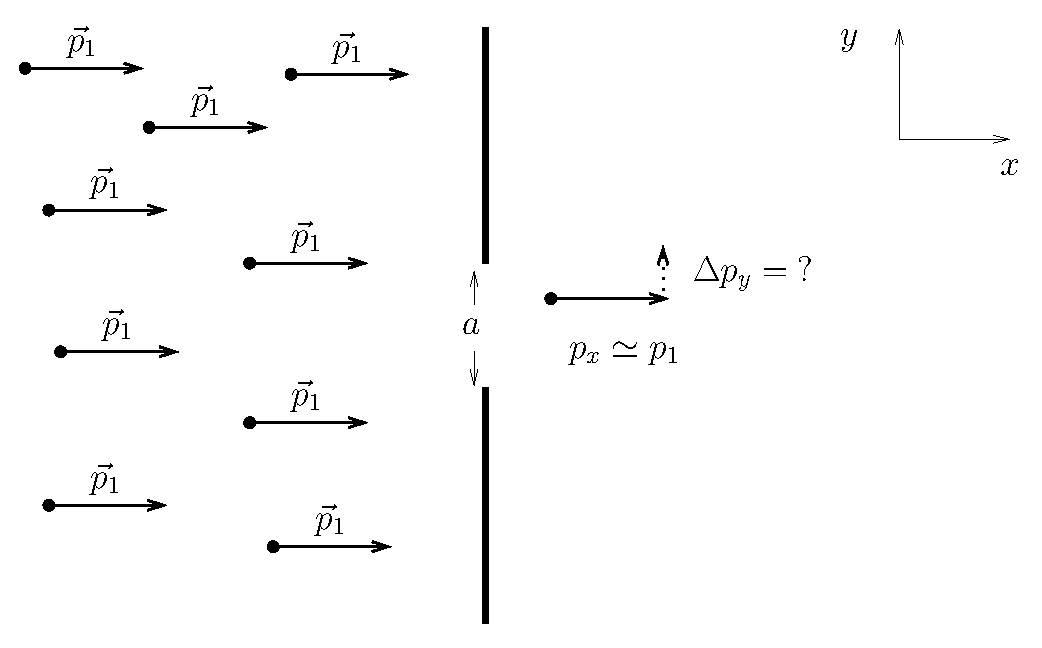
\includegraphics{additional_problems/uncertainty}}
      \caption{Problem A\ref{prob:uncertainty}}
    \end{center}
  \end{figure}
  \begin{enumerate}
  \item What is the approximate uncertainty in the vertical position
    of the particle right after it passes through the slit? (Don't
    make this harder than it is; the answer should be obvious.)
  \item Determine the approximate minimum uncertainty in the vertical
    momentum of the particle right after it passes through the slit.
    
    \begin{figure}[h]
      \begin{center}
        \scalebox{0.35}{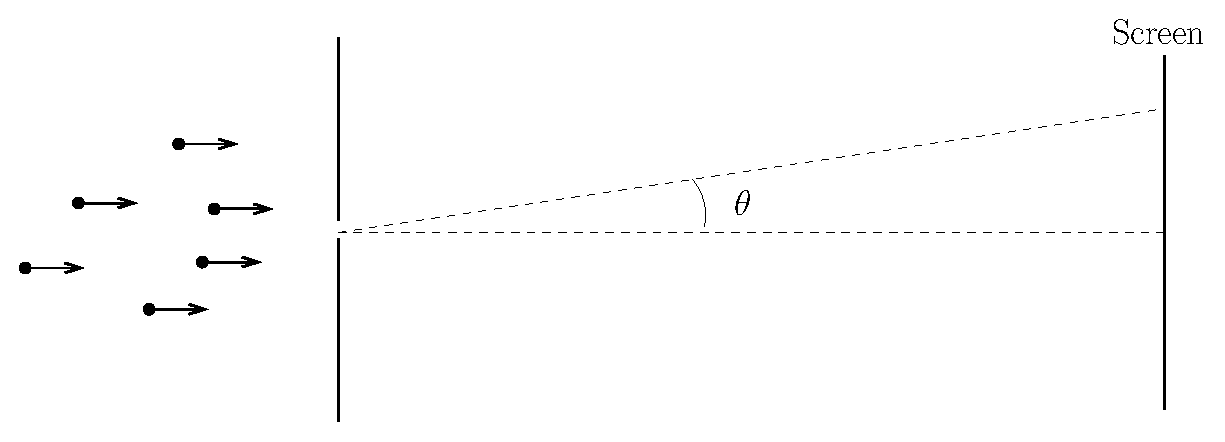
\includegraphics{additional_problems/uncertainty2}}
        \caption{Problem A\ref{prob:uncertainty}}
      \end{center}
    \end{figure}
  \item If the particle is detected on a faraway screen, show that you
    expect to find particles hit the screen over a range of angles
    $\pm \theta$, where $\theta \simeq \tan^{-1}[\lambda/(2\pi a)]$.
  \end{enumerate}
  \label{prob:uncertainty} 
\end{aproblem}


\begin{aproblem}{More uncertainty.}  
  The position of a macroscopic particle of mass $0.04\units{kg}$ is
  measured to an accuracy of $\approx 10^{-12}\units{m}$.  (This can
  actually be done using interferometers.)  Compute the minimum
  uncertainty in the velocity of the object.
  \label{prob:moreuncertainty} 
\end{aproblem}

\newpage

\begin{aproblem}{Magic Springs and the Particle-in-a-Box.}  
  Hold both ends of your Magic Spring, and get standing waves in the
  first, second, and third lowest frequency modes.  Sketch the wave
  patterns and compare them to the wave functions for the three lowest
  energy states of a ``particle in a box.''
\end{aproblem}

\begin{aproblem}{Schr\"odinger equation for a classically allowed
situation.}  
  Consider a particle of mass $m$ in a region in which the potential
  energy is constant, i.e., $U(x)=U_0$, and assume that the total
  energy of the particle $E$ is greater than the potential energy,
  i.e., $E>U_0$.  (This is the case for classically allowed motion.)
  To determine the wave function we must find a function $\psi(x)$
  that satisfies the one-dimensional Schr\"{o}dinger equation
  \[ -\frac{\hbar^2}{2m} \frac{d^2\psi(x)}{dx^2} + U(x)\psi(x) 
  = E\psi(x).  
  \]
  In this problem you will try three ``guesses'' for $\psi(x)$ and see
  if they satisfy the Schr\"{o}dinger equation. The three ``guesses''
  are
  \begin{itemize}
  \item $\psi_1(x) = Ax^2$ 
  \item $\psi_2(x) = B\sin(kx)$
  \item $\psi_3(x) = Ce^{-\kappa x}$,
  \end{itemize}
  where $A$, $B$, $C$, $k$, and $\kappa$ are undetermined real
  constants.
  \begin{enumerate}
  \item Rearrange the Schr\"{o}dinger equation so that the second
    derivative $d^2\psi/dx^2$ is alone on the left.
  \item Plug $\psi_1(x)$ into the Schr\"{o}dinger equation and see if
    there is any choice for the constant $A$ that will make
    $\psi_1(x)$ satisfy the equation for all values of $x$.
  \item Plug $\psi_2(x)$ into the Schr\"{o}dinger equation and see if
    there is any choice for the constants $B$ and $k$ that will make
    $\psi_2(x)$ satisfy the equation for all values of $x$ .
  \item Plug $\psi_3(x)$ into the Schr\"{o}dinger equation and see if
    there is any choice for the constants $C$ and $\kappa$ that will
    make $\psi_3(x)$ satisfy the equation for all values of $x$.
  \item You should have found that $\psi_2(x)$ can be a solution for
    the proper choice of $k$.  Determine the wavelength of the
    oscillations in terms of $\hbar$, $m$, $E$, and $U_0$. (i.e.,
    solve for $k$ and remember from the waves unit that
    $k=2\pi/\lambda$.)  Is your result consistent with that predicted
    from the de~Broglie relationship?  (Hint: $E-U_0$ is the kinetic
    energy $K = p^2/2m$.  Re-write things in terms of the momentum and
    the answer should drop into your lap.)
  \end{enumerate}
\end{aproblem}


\begin{aproblem}{Schr\"odinger equation for classically forbidden
situation.}  
  Consider a particle of mass $m$ in a region with a constant
  potential energy $U_0$, and assume that the total energy of the
  particle $E$ is {\em less} than the potential energy, i.e., $E<U_0$.
  (This isn't possible for classical motion, but continue anyway.)  To
  determine the wave function we must find a function $\psi(x)$ that
  satisfies the one-dimensional Schr\"{o}dinger equation
  \[ -\frac{\hbar^2}{2m} \frac{d^2\psi(x)}{dx^2} + U(x)\psi(x) 
  = E\psi(x).  
  \]
  In this problem you will try three ``guesses'' for $\psi(x)$ and see
  if they satisfy the Schr\"{o}dinger equation. The three ``guesses''
  are
  \begin{itemize}
  \item $\psi_1(x) = Ax^2$ 
  \item $\psi_2(x) = B\sin(kx)$
  \item and $\psi_3(x) = Ce^{-\kappa x}$,
  \end{itemize}
  where $A$, $B$, $C$, $k$, and $\kappa$ are undetermined real
  constants.
  \begin{enumerate}
  \item Rearrange the Schr\"{o}dinger equation so that the second
    derivative $d^2\psi/dx^2$ is alone on the left.
  \item Plug $\psi_1(x)$ into the Schr\"{o}dinger equation and see if
    there is any choice for the constant $A$ that will make
    $\psi_1(x)$ satisfy the equation for all values of $x$.
  \item Plug $\psi_2(x)$ into the Schr\"{o}dinger equation and see if
    there is any choice for the constants $B$ and $k$ that will make
    $\psi_2(x)$ satisfy the equation for all values of $x$.
  \item Plug $\psi_3(x)$ into the Schr\"{o}dinger equation and see if
    there is any choice for the constants $C$ and $\kappa$ that will
    make $\psi_3(x)$ satisfy the equation for all values of $x$.
  \end{enumerate} 
\end{aproblem}

\begin{aproblem}{Tunneling and time-energy uncertainty.}  
  Consider an electron hitting a barrier.  Assume the electron has an
  energy $E = 50\units{eV}$, and the barrier has a height $U =
  100\units{eV}$.  Semi-classically, to tunnel through the barrier,
  the electron must ``borrow'' enough energy to get over the barrier,
  and must hold this energy long enough to travel the width of the
  barrier.  The best-case scenario is if the energy fluctuates up to a
  value of $2U - E$ or $150\units{eV}$.  (See ``Optional problem''
  below if you want to see where this comes
  from.) \label{prob:tunneltime}

  \begin{enumerate}
  \item Using the energy-time uncertainty relation $\Delta E \Delta t
    \approx \hbar$, approximate the typical duration of the energy
    fluctuation (i.e., determine $\Delta t$).
  \item Determine the classical velocity of the electron in the
    barrier region if it has an energy of $150\units{eV}$.  (Warning:
    the kinetic energy of the electron is not $150\units{eV}$ here.)
  \item Determine the maximum width $L$ of the barrier such that the
    electron will make it through in a time $\Delta t$.
  \item The width $L$ that you have just determined is a width for
    which you would expect a reasonable probability for an electron to
    tunnel through a barrier.  You can calculate the transmission
    probability $T$ explicitly by $T = e^{-2\alpha L}$, where $\alpha
    = \sqrt{2m(U-E)/\hbar^2}$.  Use your value of $L$ and the
    information given above to verify that you get a reasonable value
    for $T$. (by ``reasonable,'' we mean that you should get a
    probability greater than 0.1, but, of course, it must be less than
    1.)
  \end{enumerate}
\end{aproblem}


\begin{aproblem}{Optional for mathophiles \dots} 
  (You don't have to hand this in.)  For the preceding ``A'' problem,
  show that the semi-classical approach discussed for tunneling gives
  the largest value of the barrier width $L$ if the particle borrows
  enough energy $\Delta E$ to get to an energy of $(2U - E)$. Hint:
  Use the approach from the previous problem to find the maximum
  barrier width $L$ if the particle fluctuates up to an energy of
  $E_{\rm high}$.  Then take the derivative $dL/dE_{\rm high}$ and set
  this equal to zero to figure out the optimal $E_{\rm high}$.  Note:
  conceptually, the optimal energy is a small enough energy such that
  $\Delta t$ is relatively long, but large enough such that the
  electron still has some kinetic energy while traveling across the
  barrier.
\end{aproblem}


\begin{aproblem}{Semi-infinite square-well potential.} 
  Download the Excel worksheet \verb+semi-finite.xls+ from either the
  {\it Handouts} page or from the Calendar page.  This sheet shows the
  calculations for determining the wavefunctions for a potential well
  that is infinite at $x=0$ but of finite magnitude on the right side
  of the well (which is at $x=5$ in this problem).  You'll see two
  graphs: the top one shows the semi-infinite potential well (in
  purple) along with a non-normalized plot of the calculated
  wavefunction so you can see it along with the potential.  The bottom
  graph shows the normalized wavefunction, corresponding to the
  second-to-last column in the worksheet.

  When you bring up the worksheet, the energy will be set for the
  value for the ground state.  Some questions:

  \begin{enumerate}

  \item Sketch or print out (just the first page!) the wavefunctions
    that are displayed for the ground state along with at least two of
    the excited states.  To display the 1$^{\rm st}$ and $2^{\rm nd}$
    excited states, type in 0.64282 and 1.4144 respectively in the
    framed box for energy.

  \item What happens if you type in an energy that {\bf isn't} one of
    the well-defined energies for the problem?  Try it out, and
    comment on what happens.  Had we not told you what the allowed
    energies were, how might you figure them out?  (You'll be doing
    this in lab later this semester.)  {\bf Continued} $\rightarrow$

  \item For any of the allowed states, show that the state plotted in
    the bottom graph is normalized.  Hint: we have already created a
    column for the square of the normalized wavefunction (the
    right-most column).  You might want to take advantage of the
    \verb+sum(start:end)+ routine in Excel.

  \end{enumerate}
\end{aproblem}

\begin{aproblem}{Classically allowed and classically forbid\-den
probabilities.}  
  Load the \verb+semi-finite.xls+ worksheet (the same one from the
  previous problem).  The ground state should be displayed initially.
  \begin{enumerate}
  \item If a measurement were done on this system, what would be the
    probability that the particle would be found in the region $x <
    5$?  Explain briefly how you calculated this from the Excel
    worksheet. \\ {\bf Hint:} Remember that for a continuous
    wavefunction $\psi(x)$, the probability of finding the particle in
    a particular region is\\ $\int_{x_1}^{x_2} P(x)\, dx = \int |\psi
    (x)|^2\, dx$.  However, we don't actually have a wave function to
    integrate; we have a numerical solution instead.  But we can do a
    {\it Riemann Sum} and add up the contributions: $\sum_i P(x_i)\,
    \Delta x = \sum |\psi(x_i)|^2\, \Delta x$. You'll have to
    determine what $\Delta x$ is in this Excel worksheet.
  \item What would be the probability that the particle would be found
    in the region $x > 5$?
  \item What would be the answer to questions (a) and (b) if this was
    a classical particle in a semi-infinite square-well potential with
    energy less than $U_0$ (i.e., no quantum effects)?
  \item Answer questions (a) and (b) again, but for the second excited
    state (with $E = 1.4144$).  Compare your answers with those for
    the ground state.  Do the results make sense, considering the
    higher energy? Explain.
  \item What do you think would happen if the potential dropped back
    to 0 at $x=6$?  Would the particle remain trapped indefinitely?
    Explain why or why not, and refer to the graphs to support your
    answer.  (You might want to sketch them or print them out.)
  \end{enumerate}
\end{aproblem}

\newpage

\begin{aproblem}{Wavefunctions and potential energy.} 
  The illustrated graph gives the wavefunction for bound state of an
  electron in some one-dimensional potential well.

  \begin{figure}[h]
    \begin{center}
      \scalebox{0.6}{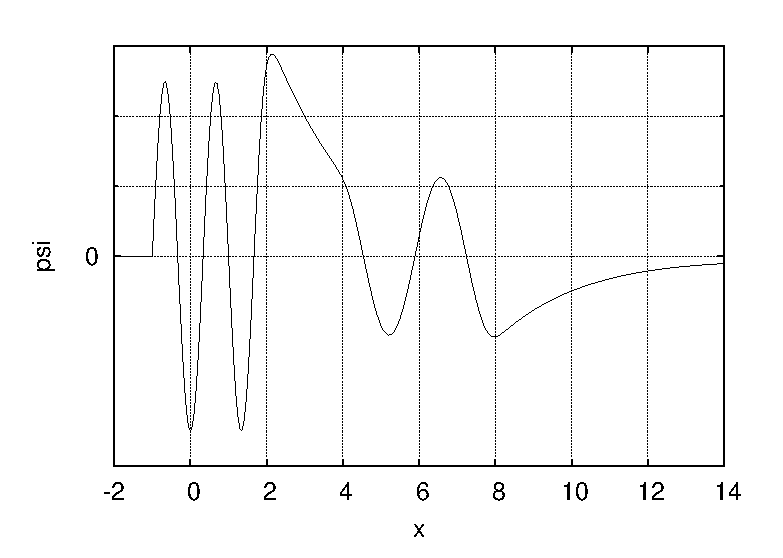
\includegraphics{additional_problems/wavefunction}}
      \caption{Problem A\ref{prob:psi-u}}
    \end{center}
  \end{figure}

  Make a qualitative sketch of the potential energy $U(x)$ versus $x$
  that could give rise to this wavefunction.  Include an indication of
  the total energy $E$ on your sketch.
  \label{prob:psi-u}
\end{aproblem}
    

\begin{aproblem}{Wavefunctions and probabilities.} 
  Using the sketch below, of the wavefunction $\psi (x)$, identify
  which letters indicate locations where the particle is: (a) most
  likely to be found and (b) least likely to be
  found. \label{prob:wavefn}

  \begin{figure}[h]
    \begin{center}
      \scalebox{0.5}[0.75]{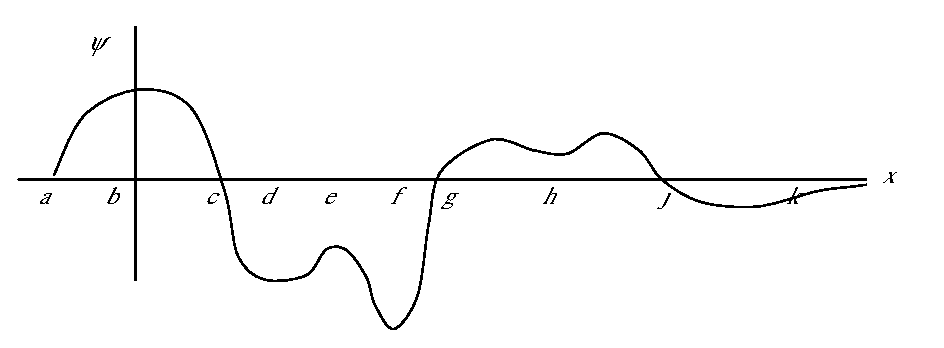
\includegraphics{additional_problems/wavefunction2}}
      \caption{Problem A\ref{prob:wavefn}}
    \end{center}
  \end{figure}
\end{aproblem}


\begin{aproblem}{Barrier tunneling:  Calculating approximate
probabilities.}  
  A $15\units{eV}$ electron is incident on a potential barrier of
  height $22\units{eV}$ and width of $0.05\units{nm}$.

  \begin{enumerate}
  \item Use the transmission probability discussed in part (d) of
    Problem A\ref{prob:tunneltime} to estimate the order of magnitude
    of the probability that the electron will tunnel through the
    barrier.
  \item If one million electrons with energy $15\units{eV}$ hit this
    barrier, roughly how many of them would you expect to get through?
  \item Repeat parts (a) and (b) for a barrier width of
    $0.5\units{nm}$.
  \end{enumerate}
\end{aproblem}


\begin{aproblem}{Annoying your roommate, Part 2} or {\bf Superposition
of states.} 
  Take your slide whistle and with the slide most or all the way out,
  blow gently into the whistle.  As we discussed in the previous unit,
  the note that you hear is due to the fundamental mode of the slide
  whistle.  If you blow harder, the pitch will jump to a higher value,
  corresponding to the second standing-wave mode.

  It is possible to blow hard enough -- but not too hard -- such that
  you hear two notes at the same time.  Do this, and comment on what
  you hear.  Now, consider the analogous quantum problem.  If these
  were two matter waves instead of sound waves, what would the
  different pitches that you hear correspond to?
\end{aproblem}


\begin{aproblem}{Life in a quantum world.} 
  Last semester we asked you to describe some relativistic effects
  that you would notice if the physical ``speed limit'' of light were
  $4\units{mph}$ instead of $3 \times 10^8\units{m/s}$. Now imagine
  that the quantum constant $\hbar$ were 1 Joule-sec.
  \begin{enumerate}
  \item The uncertainty principle in this world would be $\sigma_x
    \sigma_p \geq \frac{1}{2}\units{kg$\cdot$m$^2$/s}$.  Imagine that
    someone throws a ball to you. Describe what you would experience
    trying to catch the ball.
  \item Consider the energy of a photon.  With light frequencies still
    in the $10^{14}\units{Hz}$ range, describe how it would feel to be
    sunbathing on a beach.
  \item What would your approximate de~Broglie wavelength be when
    walking? What would happen when you walk through a doorway?
  \end{enumerate}
\end{aproblem}

\newpage

\begin{aproblem}{Transitions.}  
  The sketches below show the state of a two-level atom and possibly a
  photon.  For each ``Before'' sketch make a corresponding ``After''
  sketch and name the process.
  \label{prob:transition}

  \begin{figure}[h]
    \begin{center}
      \scalebox{0.5}{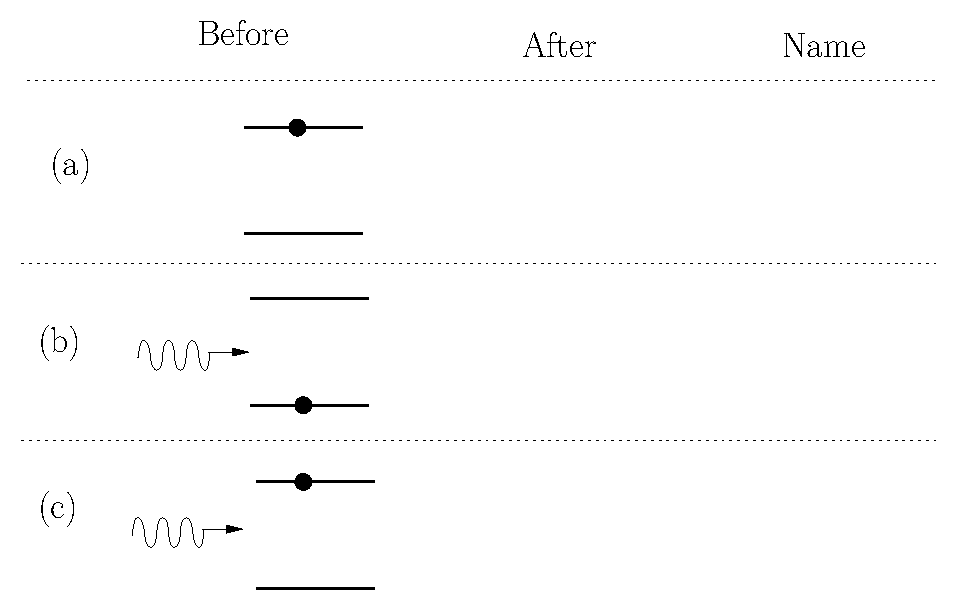
\includegraphics{additional_problems/transitions}}
      \caption{Problem A\ref{prob:transition}}
    \end{center}
  \end{figure}
\end{aproblem}


\begin{aproblem}{Population inversion.} 
  Explain briefly why a population inversion is necessary for the
  operation of a laser.
\end{aproblem}


\begin{aproblem}{Superconductors.} 
  (Do in Problem Session) Here we investigate some magnetic properties
  of superconductors.
  \begin{enumerate} 
  \item Closely observe the little cube hovering over the
    disk. Comment on what you observe.  What evidence do you have that
    this is a superconductor?  Can you make the cube spin?
  \item Explain how the superconductor can levitate the magnet.
  \end{enumerate}
\end{aproblem}


\begin{aproblem}{Flipping magnets.} 
  Find a friend to help you explore magnetic resonance. Take your
  magnet and tie string around it so it is supported in the center and
  hangs horizontally when you hold the string above and below the
  magnet.  Have your friend bring his/her magnet nearby and note that
  your magnet tries to align.  Keeping the string fairly tight, use
  your hand to twist the magnet slightly. Are you putting energy into
  the system?  What happens when you release the magnet?  On the
  atomic scale, where does this released energy go?
\end{aproblem}


\begin{aproblem}{Electron spin resonance.}  
  What is the wavelength of a photon that will induce a transition of
  an electron spin from parallel to anti-parallel orientation in a
  magnetic field of magnitude 0.20\, T?  (From Halliday, Resnick, and
  Walker p.~1048.)
  \label{prob:spinflip}
\end{aproblem}

\newpage

\begin{aproblem}{Nuclear magnetic resonance.}
  Electromagnetic waves with frequency $f = 34\units{MHz}$ illuminate
  a sample that contains hydrogen atoms.  Resonance is observed when
  the strength of the constant external magnetic field equals 0.78\,
  T.  Calculate the strength of the local magnetic field at the site
  of the protons that are undergoing spin flips, assuming the external
  and local fields are parallel there.  (adapted from Halliday,
  Resnick, and Walker p.~1048.)
  \label{prob:nmr}
\end{aproblem}


\begin{aproblem}{Flipping inside atoms.}  
  The proton, like the electron, has a spin quantum number $s$ of 1/2.
  In the hydrogen atom in its ground state ($n = 1$ and $l = 0$),
  there are two energy levels, depending on whether the electron and
  proton spins are parallel or anti-parallel.  If the electron of an
  atom has a spin flip from the state of higher energy to that of
  lower energy, a photon of wavelength 21\, cm is emitted.  Radio
  astronomers observe this 21\, cm radiation coming from deep
  space. What is the effective magnetic field (due to the magnetic
  dipole moment of the proton) experienced by the electron emitting
  this radiation?  (From Halliday, Resnick, and Walker p.~1048.)
\end{aproblem}


\begin{aproblem}{MRI.} 
  Assume that the magnetic field along a line passing through a
  patient's brain in an MRI scan is described by the function $B(x) =
  0.5 + 0.6x$, where $B$ is in Tesla and $x$ is in meters.

  \begin{enumerate}
  \item What is the location in the brain where protons will flip in
    response to a 30\, MHz oscillating magnetic field?  (Give your
    answer as $x = \mbox{\underline{\hspace{0.2in}}}\units{m}$.)
  \item If you want to probe a possible tumor at a position of $x =
    0.50\units{m}$, at what frequency should you oscillate the
    magnetic field?
  \item For your answer in part (b), what is the energy of the photons
    that are probing your patient (in eV)?  Considering that the
    weakest molecular bonding energies are around 0.1\, eV, is this
    safe for your patient?
  \end{enumerate}
\end{aproblem}


\begin{aproblem}{Particle decay.}  
  This exercise simulates the conversion of rest and kinetic energies
  in a particle decay. Take 10 coins (or any 10 objects -- pencils,
  bottle caps, small elephants, ...) and lump them together on a table
  or desktop. Each item represents 1 unit of energy.

  \begin{enumerate}
  \item Assume your pile represents a single massive particle with $m
    = 10$ in some units.  Now assume this particle decays in to 2
    particles with mass 5 and 4 units.  Split your pile up into these
    two particles.  How many extra items are left?  What do these
    extra items represent?

  \item Start again with a single pile representing a single particle
    of rest energy 10 units.  Now have the particle decay into two
    particles, one of rest energy 5 units, the other of 6 units.  (No
    borrowing from friends!)  Why can't you have a decay result in a
    larger total rest energy?

  \end{enumerate}
\end{aproblem}


\begin{aproblem}{Exchanging virtual particles.} 
  (OPTIONAL): Find a friend and a pen.  The pen represents a virtual
  force carrier (messenger particle) that will be exchanged between
  you and your friend.

  \begin{enumerate}
  \item Hold a pen in one hand, aiming the point of the pen toward
    your friend.  The direction the pen points is the direction of the
    momentum of the messenger.  Now give the pen to your friend and
    conserve momentum.  To do this, you should each modify your motion
    to reflect the momentum exchange.  For example, if you give away
    leftward momentum, you must move rightward to compensate. Describe
    your relative motions after the exchange of pen.

  \item Repeat, but have the pen initially pointing away from your
    friend.

  \end{enumerate}
\end{aproblem}


\begin{aproblem}{The expanding universe.}  
  Take a balloon and draw some stars, planets, and galaxies on the
  surface of the deflated balloon.
  \begin{enumerate}
  \item Now blow up the balloon and watch how the distance between
    adjacent galaxies changes as the universe expands.  Record your
    observations.
  \item With the balloon partially inflated, choose a reference
    galaxy.  Find two objects nearby, with one about as twice as far
    from the reference galaxy as the other.  Measure the distance.
    Then blow up the balloon and measure the distances again.  How do
    their rates of change of distance compare?  Compare this to
    Hubble's Law.
  \end{enumerate}
\end{aproblem}


\begin{aproblem}{A moving wave.}
  A wave is described by $\psi(z,t) = 5 \cos\left(\pi z/2 + \pi
  t/4\right)$, where $z$ is in meters, and $t$ is in seconds.
  \begin{enumerate}
  \item Plot $\psi$ versus $z$ at time $t=0$ between $z = -3$ and $z =
    3$.  Make another plot of $\psi$ versus $z$ at time
    $t=1\units{s}$.
  \item Find a point of zero displacement at $t=0$.  Where is this
    point of zero displacement at time $t=1\units{s}$?  (Take into
    consideration the direction the wave is traveling.)
  \item Use your answers to parts (a) and (b) to calculate the speed
    of the wave.  Does your answer agree with the speed determined
    from $\omega/k$?
  \end{enumerate}
\end{aproblem}

\newpage

\begin{aproblem}{Two antennas.}
  Two antennas are $\lambda/4$ apart.  Each emits a wave with the same
  amplitude and the same phase.  A receiver is located far away from
  the antennas, but is placed such that the receiver and the antennas
  fall on a single straight line.  Individually, each antenna gives a
  wave of amplitude $A$ at the receiver.  Calculate, in terms of $A$,
  the total amplitude at the receiver when both antennas are emitting.
  \label{prob:TwoAntennas}
\end{aproblem}


\begin{aproblem}{Find the third maximum.}
  Laser light of wavelength $633\units{nm}$ shines on a double slit
  arrangement with a slit separation of $0.003\units{mm}$.  The
  interference pattern is viewed on a screen several meters away.  At
  what angle $\theta$ does one observe the third maximum away from the
  central maximum?
\end{aproblem}

\begin{aproblem}{Two loudspeakers.}
  Two loudspeakers, $3.0\units{m}$ apart, are driven at the same
  frequency and in phase.  They emit sound with a wavelength of
  $2.0\units{m}$.
  \label{prob:speakers}
  \begin{figure}[h]
    \begin{center}
      \scalebox{0.7}{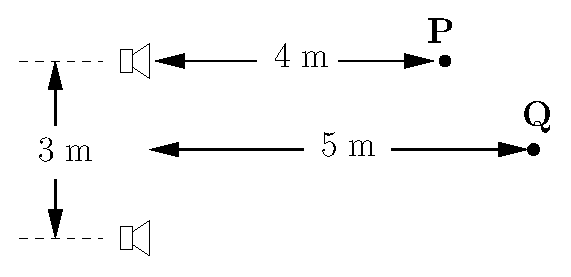
\includegraphics{additional_problems/speakers}}
      \caption{Problem A\ref{prob:speakers}}
    \end{center}
  \end{figure}
  \begin{enumerate}
  \item Point {\bf P} is $4.0\units{m}$ from the line joining the
    speakers and is directly in front of one speaker.  Is the
    intensity at {\bf P} a maximum, a minimum, or neither?
  \item Point {\bf Q} is $5.0\units{m}$ from the midpoint between the
    speakers and equidistant from them.  The intensity at {\bf Q} when
    only one speaker is on is $I_0$, and when only the other speaker
    is on the intensity at {\bf Q} is $4I_0$.  Find the intensity at
    {\bf Q} when both speakers are on.
  \end{enumerate}
\end{aproblem}


\begin{aproblem}{Three loudspeakers.}
  Three loudspeakers are arranged on a line and separated by
  $3.0\units{m}$, as shown in Fig.~\ref{fig:speakers2}. They are
  driven at the same frequency and in phase.  They emit sound with a
  wavelength of $2.0\units{m}$.  Point {\bf P} is $4.0\units{m}$ from
  the line joining the speakers and is directly in front of the
  central speaker.  The sound intensity at {\bf P} when any one
  speaker is on is $I_0$.
  \label{prob:speakers2} 
  \begin{figure}[h]
    \begin{center} 
      \scalebox{0.65}{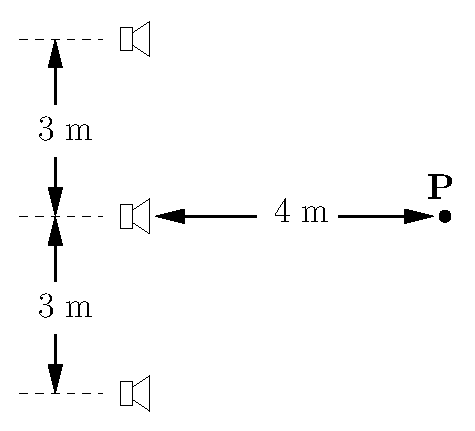
\includegraphics{additional_problems/speakers2}}
      \caption{Problem A\ref{prob:speakers2}}
      \label{fig:speakers2}
    \end{center}
  \end{figure}
  \begin{enumerate}
  \item Draw a phasor diagram representing the sound waves at point
    {\bf P}.  Include a phasor for the wave from each speakers, and a
    phasor for the total wave that results from the superposition of
    these three waves.
  \item Calculate the intensity (in terms of $I_0$) at {\bf P} when
    all three speakers are on.
  \end{enumerate}
\end{aproblem}


\begin{aproblem}{Find the formula.}
  The illustration shows two snapshots of a traveling wave, one taken
  at $t=0\units{s}$ and one taken at $t = 0.25\units{s}$.  Determine a
  formula for the function $y(x,t)$ that describes this traveling
  wave.
  \label{prob:wave_to_eq}
  \begin{figure}[h]
    \begin{center}
      \scalebox{0.65}{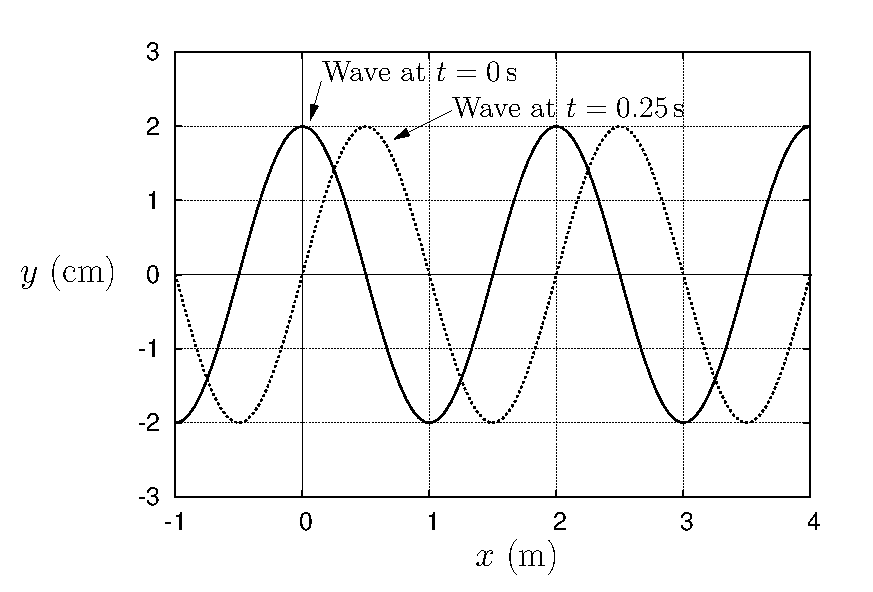
\includegraphics{additional_problems/wave_to_eq}}
      \caption{Problem A\ref{prob:wave_to_eq}}
    \end{center}
  \end{figure}
\end{aproblem}

\newpage

\begin{aproblem}{Adding waves graphically.}
  The graph in Fig.~\ref{fig:wave_to_phasor_1} shows a snapshot of two
  traveling waves at the same instant of time.  The waves have the
  same speed and frequency.  Add these two waves graphically to find
  their sum.

  \label{prob:wave_to_phasor_1}
  \begin{figure}[h]
    \begin{center}
      \scalebox{0.65}{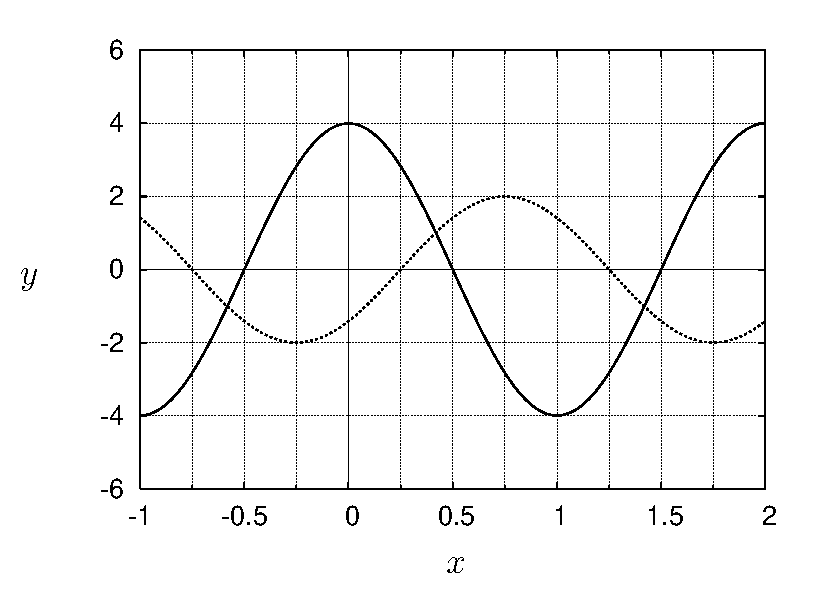
\includegraphics{additional_problems/wave_to_phasor}}
      \caption{Problem A\ref{prob:wave_to_phasor_1}}
      \label{fig:wave_to_phasor_1}
    \end{center}
  \end{figure}

  \vspace{-0.1in}
  {\bf NOTE:} There is no calculation to be performed in this
  graphical addition.  You should be thinking about this as filling in
  entries in a table like the following by reading values from the
  graph, and then plotting the last column, $y_{\rm sum}$ vs. $x$ on
  the graph.
%  \vspace{0.1in}

  \begin{center}
    \begin{tabular}{|c||c|c||c|} \hline
      $x$ & $y_{\rm solid}$ & $y_{\rm dotted}$ & $y_{\rm sum}$ \\ \hline\hline  
      -0.5  & & & \\ \hline
      -0.25 & & & \\ \hline
      0.0   & & & \\ \hline
      0.25  & & & \\ \hline
      \mbox{etc.} & & & \\ \hline
    \end{tabular}
  \end{center}
  \vspace{0.1in}
\end{aproblem}

\begin{aproblem}{Adding waves with phasors.}
  The graph in Fig.~\ref{fig:wave_to_phasor_2} shows a snapshot of two
  traveling waves at the same instant of time.  The waves have the
  same speed and frequency.
  \label{prob:wave_to_phasor_2}
  \begin{figure}[h]
    \begin{center}
      \scalebox{0.65}{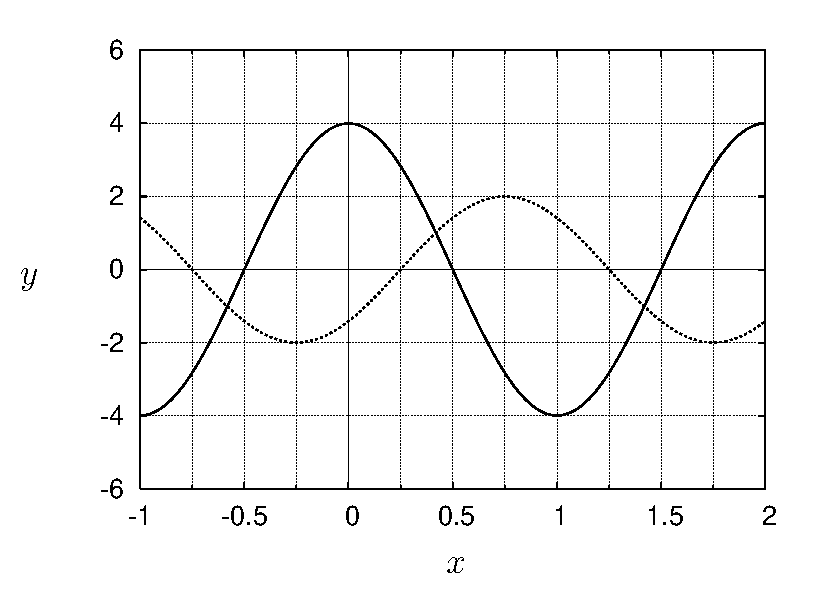
\includegraphics{additional_problems/wave_to_phasor}}
      \caption{Problem A\ref{prob:wave_to_phasor_2}}
      \label{fig:wave_to_phasor_2}
    \end{center}
  \end{figure}

  \begin{enumerate}
  \item Draw two phasors representing these two waves.
  \item Calculate the amplitude of the superposition of these waves.  
  \item Calculate the phase shift of the resultant wave
    with respect to solid wave in the illustration.
  \item Compare your resultant amplitude and phase with the 
    graphical result you got in Problem A\ref{prob:wave_to_phasor_1}.	
  \end{enumerate}
\end{aproblem}


\begin{aproblem}{ Parking Lot.}  
  John, the aspiring physics student/parking attendant (see
  Supp. Ch. 3, Problem \# \ref{prob:parking_lot_1}) gets a job at a
  new hotel that has a more conventional parking lot.  The parking lot
  has a rectangular shape on an $x$-$y$ coordinate system with
  dimensions $100\units{m}\times 50\units{m}$, and the lot is divided
  into three sections, {\bf A}, {\bf B}, and {\bf C} (see figure).
  Although the lot is more conventional, John still tells car owners
  the whereabouts of their cars in terms of probabilities and
  probability densities, only now the probability densities are given
  in terms of {\em probability per unit area} instead of of {\em
    probability per unit length}, and they are functions of two
  variables, $x$ and $y$.
  \label{prob:parking_lot_2}
  \begin{figure}[h]
    \begin{center}
      \scalebox{0.65}{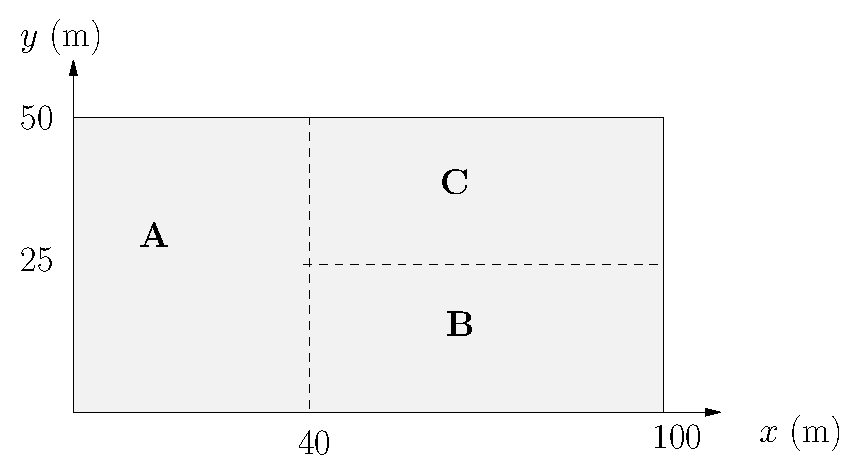
\includegraphics{additional_problems/parking_lot_2}}
      \caption{Problem A\ref{prob:parking_lot_2}}
    \end{center}
  \end{figure}

  \begin{enumerate}
  \item Mr.~Vanderbilt is told that his car ``could be anywhere in the
    lot,'' which means that the probability density is constant
    everywhere (i.e., there is no difference between the sections).
    Calculate the value of this uniform probability density $P(x,y)$
    for Mr.~Vanderbilt to find his car at a position $(x,y)$ on the
    coordinate system of the lot.  (Your answer should be in units of
    probability/m$^2$.)
  \item Find the probability that Mr.~V's car is in section {\bf A} of
    the lot.
  \item Mrs.~Reeve is told that the probability density to find her
    car is a constant $P_A$ in section {\bf A}, a second constant $P_B
    = 4P_A/3$ in section {\bf B}, and a third constant $P_C = 2P_A/3$
    in section {\bf C}.  Find the constants $P_A$, $P_B$, and $P_C$.
  \item Based on your results from part (c), calculate the probability
    that Mrs.~Reeve's car is located in the lower left quarter of the
    lot, i.e, in the region where $0\leq x\leq 50$ and $0\leq y \leq
    25$.
  \end{enumerate}
\end{aproblem}

\begin{aproblem}{Daughter of parking lot.}  
  John, the aspiring physics student/parking attendant (see Problems
  Supp. Ch.~3 \#\ref{prob:parking_lot_1} and {\bf
    A\ref{prob:parking_lot_2}}) gets a job at %yet another hotel, and
  this one has a circular parking lot with radius $40\units{m}$ laid
  out on a $r$-$\theta$ polar coordinate system, and the lot is
  divided into two sections, {\bf A} and {\bf B}.
  \label{prob:parking_lot_3}
  \begin{figure}[h]
    \begin{center}
      \scalebox{0.65}{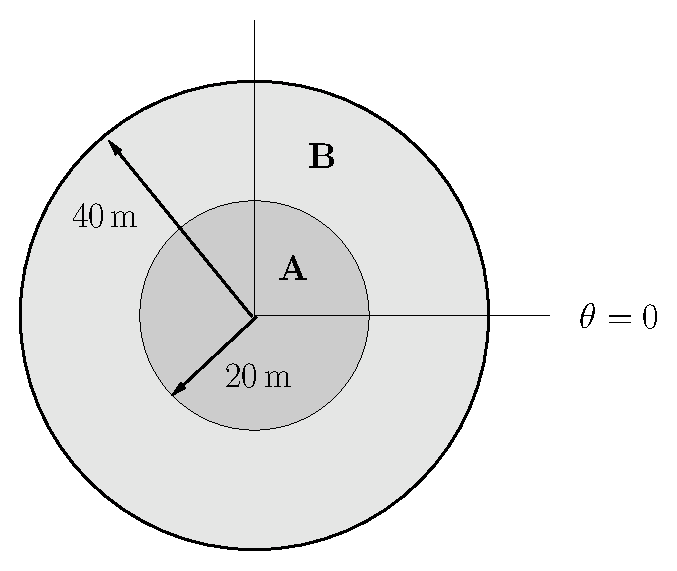
\includegraphics{additional_problems/parking_lot_3}}
      \caption{Problem A\ref{prob:parking_lot_3}}
    \end{center}
  \end{figure}

  \begin{enumerate}
  \item Mr.~Vanderbilt is told that his car ``could be anywhere in the
    lot,'' which means that the probability density is constant
    everywhere (i.e., there is no difference between the sections).
    Calculate the value of this uniform probability density
    $P(r,\theta)$ for Mr.~Vanderbilt to find his car at a position
    $(r,\theta)$ on the coordinate system of the lot.  (Your answer
    should be in units of probability/m$^2$.)
  \item Find the probability that Mr.~V's car is in section {\bf A} of
    the lot.
  \item Mrs.~Reeve is told that the probability density to find her
    car is a constant $P_A$ in section {\bf A} and a second constant
    $P_B = P_A/2$ in section {\bf B}.  Find the constants $P_A$ and
    $P_B$.
  \item Based on your results from part (c), calculate the probability
    that Mrs.~Reeve's car is located within $30\units{m}$ of the
    center of the lot.
  \end{enumerate}
\end{aproblem}


\begin{aproblem}{More practice with complex numbers.}
  \begin{enumerate}
  \item Given the number $z_1 = 0.25$, determine the complex conjugate
    of $z_1$, i.e., determine $z_1^\ast$.
  \item Given the number $z_2 = 0.25i$, determine the complex
    conjugate of $z_2$, i.e., determine $z_2^\ast$.
  \item Given the number $z_3 = 0.5 + 0.3i$, determine the
    magnitude-squared of $z_3$, i.e., determine $\vert z_3\vert^2$.
  \end{enumerate}
\end{aproblem}


\begin{aproblem}{Practice with the complex exponential.}  
  This is a series of exercises that review material from your
  calculus courses, and to give you practice with imaginary numbers in
  an exponent.  Recall from your calculus classes the following Taylor
  series expansions:
  \label{prob:ComplexPractice}
  \begin{eqnarray}
    e^x &=&  1+ x +\frac{x^2}{2!}+\frac{x^3}{3!}+ \frac{x^4}{4!} + \cdots
    \nonumber \\
    \cos x &=& 1 - \frac{x^2}{2!} + \frac{x^4}{4!} + \cdots 
    \nonumber \\
    \sin x &=&  x- \frac{x^3}{3!} + \frac{x^5}{5!} + \cdots
    \nonumber 
  \end{eqnarray}
  
  \begin{enumerate}
  \item Use the expansion for $e^x$ from above, and write a series for
    expression for $e^{i\theta}$, where $\theta$ is a real number.  In
    your answer, don't leave any $i^2$, $i^3$ or $i^4$ factors, (i.e.,
    substitute in the result that $i^2=-1$ whenever possible).

  \item Regroup the terms in your answer from part (a) to show that
    \[  e^{i\theta}=\cos\theta +i\sin\theta.  \]

  \item Use the expansion for $e^x$ from above, and write a series for
    expression for $e^{-i\theta}$, where $\theta$ is a real number.
    In your answer, don't leave any $i^2$, $i^3$ or $i^4$ factors,
    (i.e., substitute in the result that $i^2=-1$ whenever possible)

  \item Regroup the terms in your answer from part (c) to show that
    \[  e^{-i\theta}=\cos\theta - i\sin\theta.  \]

  \item Add the expressions in for $e^{i\theta}$ and $e^{-i\theta}$
    from the results of parts (b) and (d) to show that
    \[ \cos\theta = \frac{e^{i\theta} + e^{-i\theta}}{2}. \]

  \item Find the difference of the expressions for $e^{i\theta}$ and
    $e^{-i\theta}$ from the results parts (b) and (d) to show that
    \[ \sin\theta = \frac{e^{i\theta} - e^{-i\theta}}{2i} = 
    \frac{-i}{2}\left(e^{i\theta} - e^{-i\theta}\right). \]

  \item Write the number $e^{0.5i}$ in the form $a + ib$, where $a$
    and $b$ are real numbers.

  \item Write the number $e^{-0.5i}$ in the form $a + ib$, where $a$
    and $b$ are real numbers.
   
  \item Write the number $e^{0.5i} + e^{-0.5i}$ in the form $a + ib$,
    where $a$ and $b$ are real numbers.

  \item Write the number $e^{0.5i} - e^{-0.5i}$ in the form $a + ib$,
    where $a$ and $b$ are real numbers.

  \item Write the number $\cos(0.3)$ in terms of complex exponentials.

  \item Write the number $\sin(0.3)$ in terms of complex exponentials.

  \item Calculate $|e^{0.3i}|^2$.  Do this two different ways:
    \begin{enumerate}
    \item Write the complex exponential in the form $a + ib$ and find
      the magnitude-squared of this number by multiplying $a+ib$ by
      its complex conjugate.
    \item Find the complex conjugate of $e^{0.3i}$ directly (i.e.,
      leave everything in exponential form) and multiply $e^{0.3i}$ by
      this complex conjugate.
    \end{enumerate}

  \item For reference, calculate $(e^{0.3i})^2$.  (Note that this is
    just squaring rather than taking the magnitude-squared.)  How does
    your answer compare with the result of the previous part?

  \end{enumerate}
\end{aproblem}


\begin{aproblem}{Time-dependent particle-in-box.}   
  Assume that an electron is trapped in a one-dimensional box. The
  energy of the ground state ($|1\rangle$) is $E_1$ and the energy of
  the first excited state ($|2\rangle$) is $4E_1$.  At time $t=0$ the
  electron is in the state
  \[ |\psi(t=0)\rangle = \sqrt{\frac{3}{5}}|1\rangle 
  + \sqrt{\frac{2}{5}}|2\rangle.
  \]
  
  \begin{enumerate}
  \item Calculate the expectation value of the energy for the electron
    at time $t=0$.
  \item Write down the time-dependent state $|\psi(t)\rangle$ (with
    complex exponentials in the coefficients).
  \item Calculate the expectation value of the energy for the electron
    at an arbitrary time $t$.
  \end{enumerate}
  \label{prob:timedependence_1}
\end{aproblem}


\begin{aproblem}{Precessing spins I.}  
  In lecture we considered a particle like a proton (with $s=1/2$ and
  magnetic moment parallel to the spin angular momentum) situated in a
  magnetic field and initially in the state $|\mbox{$+x$}\rangle$, and
  we worked out the time-dependent probabilities for measurements of
  the $x$-component of the spin angular momentum to yield $+\hbar/2$
  and $-\hbar/2$.  In this problem you will repeat the calculation
  done in lecture, but this time for measurements of the $y$-component
  of spin angular momentum.  Don't panic --- we'll take you through
  this step-by-step.
  \label{prob:qm_precess_1}

  \begin{enumerate}

  \item Assume that a particle with magnetic moment $\mu$ starts off
    at time $t=0$ in the state $|\mbox{$+x$}\rangle$; i.e., a
    measurement of $S_x$ would definitely produce a result of $+\hbar
    /2$.  Write down the state $|\psi(0)\rangle$ in terms of the
    ``spin-up'' and ``spin-down'' states $|\mbox{$+z$}\rangle$ and
    $|\mbox{$-z$}\rangle$.

  \item Now assume that the particle is in a magnetic field
    $\vec{B}=B_0 \widehat{k}$.  In a field pointing in the positive
    $z$ direction like this, the states of definite energy are
    $|\mbox{$+z$}\rangle$ and $|\mbox{$-z$}\rangle$.  Write down
    expressions for the energies of these two states.

  \item Use the energies from part (b) to write down an expression for
    the {\em time-dependent} state $|\psi(t)\rangle$.  As a
    short-hand, feel free to use the frequency $\omega \equiv 2\mu
    B_0/\hbar$.

  \item Calculate the probability that a measurement of the
    $y$-component of the spin will give a value $+\hbar/2$.

  \item Calculate the probability that a measurement of the
    $y$-component of the spin will give a value $-\hbar/2$.

  \item Show that the expectation value for measurements of the
    $y$-com\-ponent of spin angular momentum for particles in state
    $|\psi(t)\rangle$ is $(-\hbar/2)\sin(\omega t)$, where $\omega =
    2\mu B/\hbar$.

  \end{enumerate}
\end{aproblem}

\newpage

\begin{aproblem}{Time-dependence of wave functions for particle-in-box.}
  In previous chapters we discussed wavefunctions for particles rather
  than the abstract state-vector representation we have been using for
  properties like ``spin.''  The time dependence of wavefunctions can
  be handled in the same way as the time dependence of spin states.
  First, we write the wavefunction as a normalized linear combination
  of wavefunctions for states with definite energies, and each piece
  of the sum gets a factor of $e^{-iE_it/\hbar}$.  Consider a
  ``particle in a box'' that starts in a linear combination of the
  ground state and the first excited state.  The initial wavefunction
  is
  \[ \psi(t=0) =
  \sqrt{\frac{1}{L}}\sin\left(\frac{\pi x}{L}\right)+
  \sqrt{\frac{1}{L}}\sin\left(\frac{2\pi x}{L}\right), \]
  and at a later time the wave function is
  \[ \psi(t) = 
  e^{-iE_1t/\hbar}\sqrt{\frac{1}{L}}\sin\left(\frac{\pi x}{L}\right)+
  e^{-iE_2t/\hbar}\sqrt{\frac{1}{L}}\sin\left(\frac{2\pi
    x}{L}\right), \] 
  where $E_1 = \frac{h^2}{8mL^2}$ and $E_2 = \frac{h^2}{2mL^2}$ are
  the energies of the two lowest states of a particle in a box. In
  your work for parts (a) and (b) you should leave the energies as
  $E_1$ and $E_2$.

  \begin{enumerate}

  \item Determine the function $|\psi(x,t)|^2$ for the probability
    density as a function of time for this system.

  \item Compare the answer that you got for part (a) here with the
    results from Supplementary Reading Chapter 2, problem 5 and
    comment on the similarities.  (Hint: you should find that the
    answer here alternates in time between the three different
    solutions that you found in Supp.~2-5.)

  \item Download the Excel worksheet \verb+p_in_box.xls+ from the
    calendar page for Lecture 21.  This worksheet plots the
    probability density function that you found in part (b).  Try
    changing the time in the highlighted box at the top -- try $t =
    0$, 0.1, 0.2, 0.3, 0.4, 0.5, $\dots$ up through 2.1.  Comment on
    what you observe with the graphs and what these results imply
    about where you would expect to find the particle after
    measurement of position.
  \end{enumerate}
  \label{prob:time_dependent_wavefunctions}
\end{aproblem}

\newpage

\begin{aproblem}{Precessing spins II.}  
  In this problem you will complete calculations analogous to those
  you performed in problem {\bf A\ref{prob:qm_precess_1}}, except this
  time you will start with the same particle in the state
  $|\mbox{$+y$}\rangle$.

  \begin{enumerate}

  \item Assume that a spin one-half particle with magnetic moment
    $\mu$ oriented parallel to the spin starts off at time $t=0$ in
    the state $|\mbox{$+y$}\rangle$; i.e., a measurement of $S_y$
    would definitely produce a result of $+\hbar /2$.  Write down the
    state $|\psi(0)\rangle$ in terms of the ``spin-up'' and
    ``spin-down'' states $|\mbox{$+z$}\rangle$ and
    $|\mbox{$-z$}\rangle$.

  \item Now assume that the particle is in a magnetic field
    $\vec{B}=B_0 \widehat{k}$.  In a field pointing in the positive
    $z$ direction like this, the states of definite energy are
    $|\mbox{$+z$}\rangle$ and $|\mbox{$-z$}\rangle$.  Write down
    expressions for the energies of these two states.

  \item Use the energies from part (b) to write down an expression for
    the {\em time-dependent} state $|\psi(t)\rangle$.  As a
    short-hand, feel free to use the frequency $\omega \equiv 2\mu
    B_0/\hbar$.

  \item Calculate the probability that a measurement of the
    $y$-component of the spin will give a value $+\hbar/2$.
    
  \item Calculate the probability that a measurement of the
    $y$-component of the spin will give a value $-\hbar/2$.

  \item Show that the expectation value for measurements of the
    $y$-com\-ponent of spin angular momentum for particles in state
    $|\psi(t)\rangle$ is $(\hbar/2)\cos(\omega t)$, where $\omega =
    2\mu B/\hbar$.

  \end{enumerate}
\end{aproblem}

\newpage

\begin{aproblem}{Electric field from a ring of charge.}
  A ring with a radius {\it R} and total charge {\it Q} (distributed
  uniformly) lies in the x-y plane.  Determine the electric field at
  the point {\it P} on the z-axis at a height {\it h} above the center
  of the ring.  {\bf Show all the steps needed to set up and evaluate
    the integral.}
  \label{prob:efield_from_ring}
  \begin{figure}[h]
    \begin{center}
      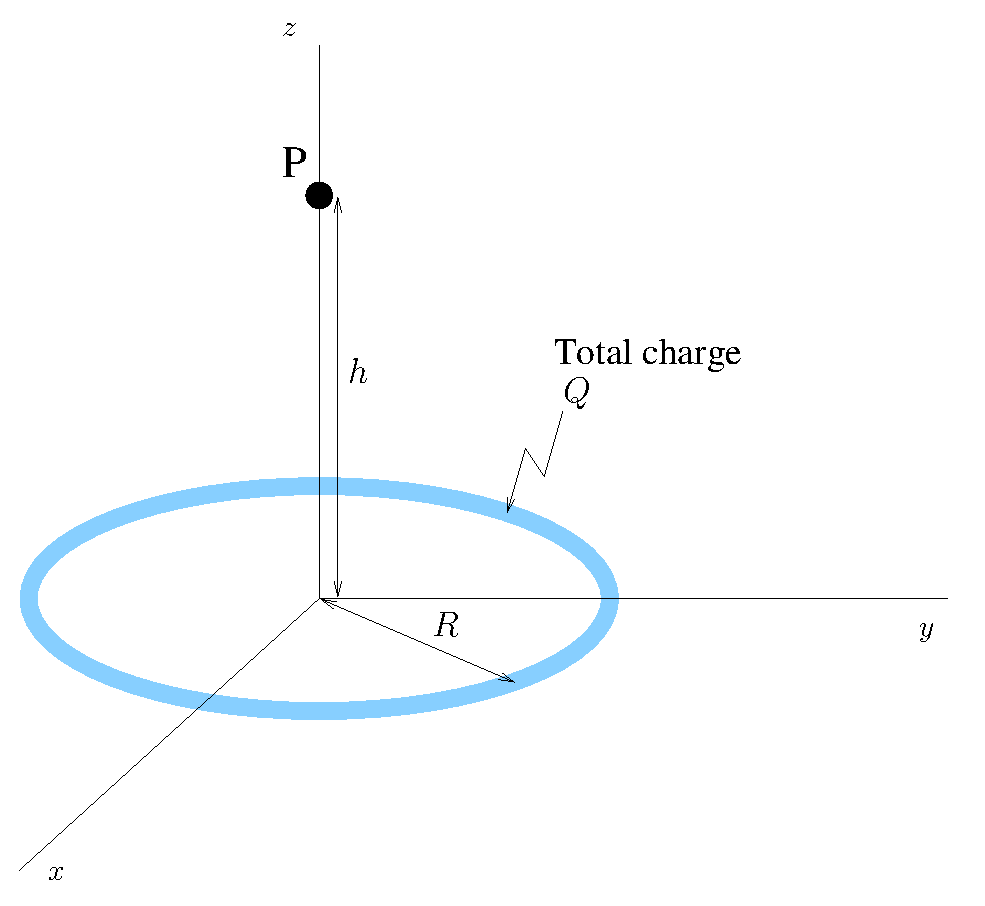
\includegraphics[width=2.4in]{additional_problems/a102fig}
      \caption{Figure for problem A\ref{prob:efield_from_ring}.}
      \label{fig:a102}
    \end{center}
  \end{figure}
\end{aproblem}

\begin{aproblem}{ Phasors and waveforms.}
  The graphs below show snapshots of two traveling waves on a string
  at the same instant of time.
  \label{prob:phasors_and_waveforms}

  \begin{center}
    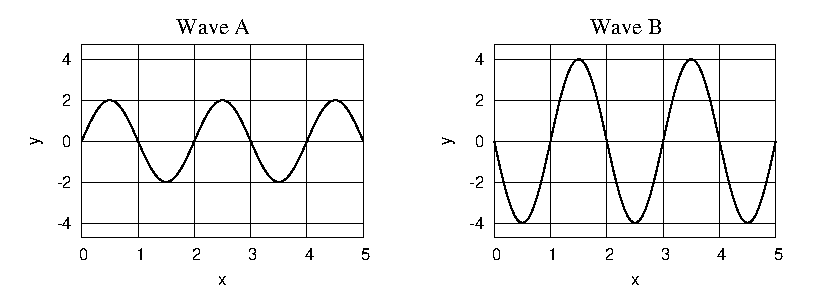
\includegraphics[width=5.0in]{additional_problems/a103fig}
  \end{center}

  \begin{enumerate}
  \item Draw a phasor diagram which represents the superposition of
    these two waves.  The diagram should be clearly labeled to show
    what represents ``Wave A,'' what represents ``Wave B,'' and what
    represents the superposition of the two (``A+B'').

  \item From the phasor diagram, determine the amplitude of the
    superposition of waves A and B.

  \end{enumerate}
\end{aproblem}

\newpage

\begin{aproblem}{Phasors and waveforms II.}
  The graphs below show snapshots of two traveling waves on a string
  at the same instant of time.

  \begin{center}
    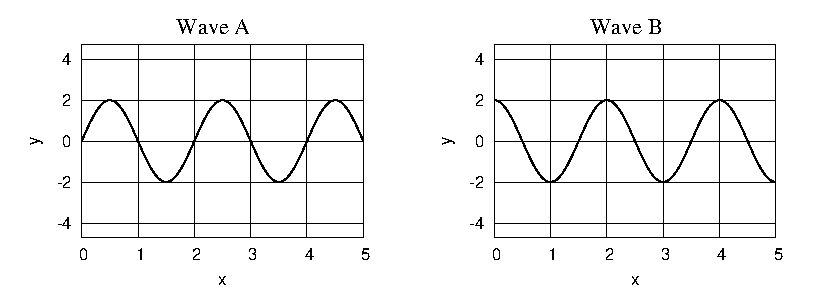
\includegraphics[width=5.0in]{additional_problems/a104fig}
  \end{center}

  \begin{enumerate}
  \item Draw a phasor diagram which represents the superposition of
    these two waves.  The diagram should be clearly labeled to show
    what represents ``Wave A,'' what represents ``Wave B,'' and what
    represents the superposition of the two (``A+B'').

  \item From the phasor diagram, determine the amplitude of the
    superposition of waves A and B.

  \end{enumerate}
\end{aproblem}


\begin{aproblem}{ Radio towers.}
  Three equally spaced AM radio towers are located to the left of a
  receiver as illustrated.  The towers broadcast in-phase radio waves
  of equal amplitude and with wavelength of 500 m.

  \vspace{2mm}
  \begin{center}
    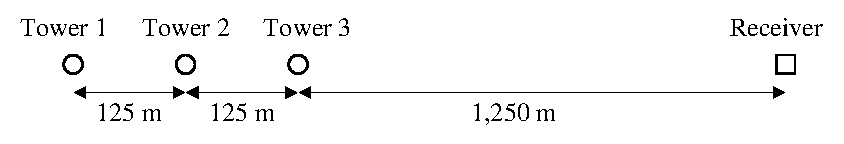
\includegraphics[width=4.5in]{additional_problems/a105fig}
  \end{center}

  \begin{enumerate}

  \item Draw a phasor diagram representing the combined radio wave at
    the receiver.

  \item Assuming the amplitude of the wave reaching the receiver from
    each tower individually is {\em A}, determine the amplitude of the
    combined wave at the receiver.
    
  \end{enumerate}
\end{aproblem}


\newpage

\begin{aproblem}{Feynman fun.}
  Fill in the missing particles (including color and/or charge labels
  where necessary) for the following three Feynman diagrams.
  \label{prob:Feynman_fun}
  \vspace{2mm}
  \begin{center}
    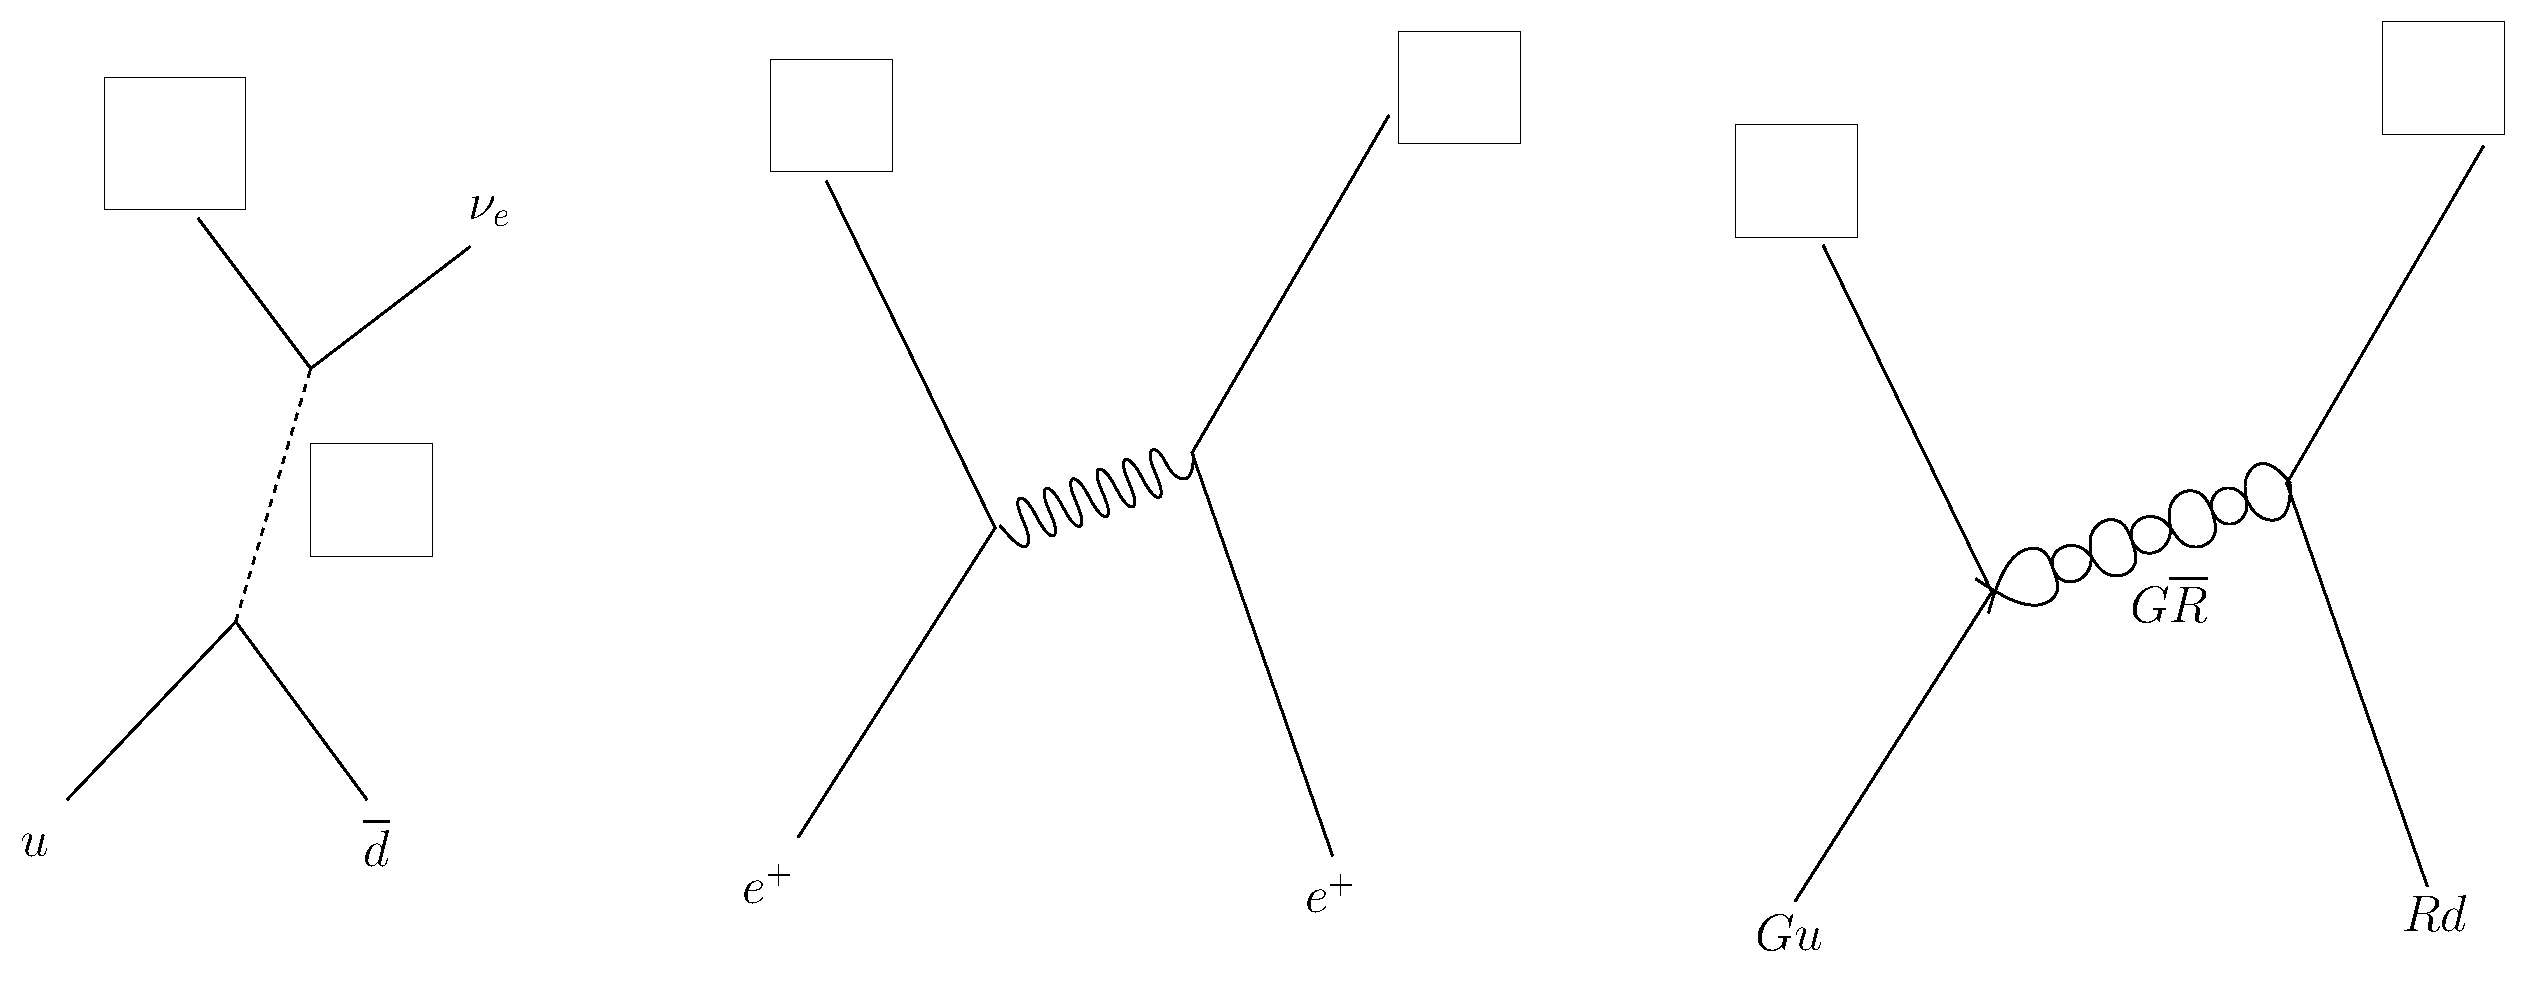
\includegraphics[width=5.4truein]{additional_problems/Feynman_fun}
  \end{center}
  \vspace{2mm}
\end{aproblem}

\begin{aproblem}{Strings and quantum mechanics.}
  This problem compares the time-dependence for a standing wave on a
  string with the time-dependence of the quantum wave function for a
  particle in a box.
  \begin{enumerate}
  \item A string of length $L$ vibrates in its 3rd lowest-frequency
    mode.  Make a sketch of this mode and then write the wavefunction
    in the form
    \[	
    \psi(x) = A \sin (kx),
    \]
    inserting the value of the wave number $k$ that you determine from
    the sketch.

  \item For waves on strings, the angular frequency $\omega$ is
    related to the wave number through $v = \omega / k$. Use this
    relation to write the time-dependent standing wave function,
    \[
    \Psi(x,t) = A \sin (kx) e^{-i\omega t},
    \]
    by expressing both $\omega$ and $k$ in terms of constants and
    properties of the string.

  \item Now consider a particle of mass $m$, confined to 1-D box of
    length $L$ in its third lowest energy state.  Make a sketch of
    this state and then write the wave function in the form
    \[
    \psi(x) = A \sin (kx),
    \]
    inserting the value of the wave number $k$ that you determine from
    the sketch.

  \item For a quantum particle, the angular frequency $\omega$ is
    related to the particle's energy by $E=\hbar\omega$.  For a
    particle free to move within the box, the energy is all kinetic:
    \[
    E=K = \frac{1}{2}mv^2 = \frac{p^2}{2m}= \frac{(\hbar k)^2}{2m}.
    \]
    Use this relation to write the time-dependent quantum
    wavefunction,
    \[
    \Psi(x,t) = A \sin (kx) e^{-iEt/\hbar}
    \]
    by expressing both $E$ and $k$ in terms of constants and
    properties of the particle and the box.
  \end{enumerate}
\end{aproblem}

\begin{aproblem}{Quantum mass-spring.}  
  A quantum mass of $2.5 \times 10^{-10}\units{kg}$ hangs from a
  quantum spring with spring constant $3.5 \times 10^{-5}\units{N/m}$.

  \begin{enumerate}
  \item Recall that classically, the classical angular frequency
    $\omega_c$ of a mass-spring system is independent of amplitude,
    and given by $\omega_c = \sqrt{k_\text{sp}/m}$.  Calculate this
    oscillator's classical period.

  \item The time-dependent quantum wavefunction for this oscillator
    depends on time as $e^{- iEt/\hbar}$ and thus also oscillates.
    Calculate the period of the \textit{wavefunction's} oscillation in
    its 3rd excited state, and compare to your answer in part (a).
  \end{enumerate}
\end{aproblem}


\begin{aproblem}{A square of charges.}
  Three identical charges $q$ and a fourth charge $-q$ form a square
  with sides of length $a$.  Find the electric force vector acting on
  a charge $Q$ placed at the center of the square.
  \label{prob:charges_on_square}

  \begin{figure}[h]
    \begin{center}
      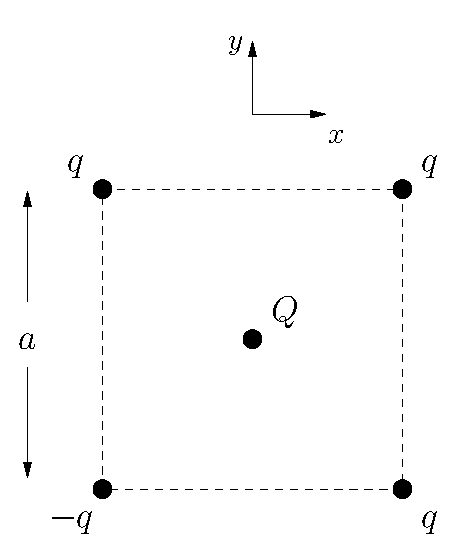
\includegraphics[width=1.75in]{additional_problems/charges_on_square}
    \end{center}
    \caption{Problem A\ref{prob:charges_on_square}.}
  \end{figure}
\end{aproblem}

\newpage

\begin{aproblem}{Parallel currents.}
  Two parallel wires oriented perpendicular to the page are separated
  by $10.0\units{cm}$.  Each wire carries a current of $1.5\units{A}$
  directed out of the page.  Determine the magnitude of the total
  magnetic field at a point {\em P} in the figure, a distance
  $12.0\units{cm}$ above the midpoint of the line connecting the two
  wires.
  \label{prob:two_wires}
  \begin{figure}[h]
    \begin{center}
      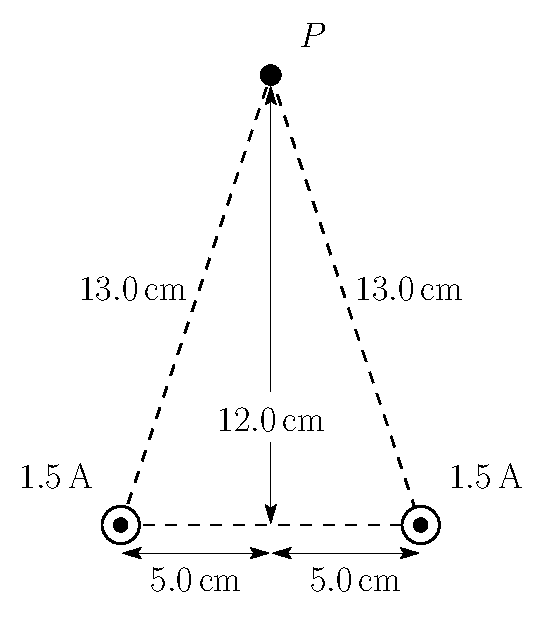
\includegraphics[width=2.in]{additional_problems/two_wires}
    \end{center}
    \caption{Problem A\ref{prob:two_wires}.}
  \end{figure}
\end{aproblem}


\begin{aproblem}{Magnetic field from a wire.}
  A long straight wire $1.0\units{cm}$ in diameter carries a current
  of $5.0\units{A}$ which is evenly distributed over its
  cross-section.  Find the magnetic field strength
  \begin{enumerate}
  \item at a point $5.0\units{mm}$ from the surface of the wire;
  \item at the surface of the wire;
  \item at a point $2.5\units{mm}$ from the axis of the wire.	
  \end{enumerate}
  \label{prob:ampere_wire}
\end{aproblem}


\begin{aproblem}{Whirly Tubes.}  
  Get out your whirly tube and give it a whirl.  Observe it is
  possible to get different notes from it, but not any frequency you
  want; only a certain frequencies seem to be allowed.  Let's
  understand where those are coming from.
  \smallskip

  Your whirly tube has a length of $75\units{cm}$ and is open at both ends.
  \begin{enumerate}
  \item Sketch the standing wave pattern for the three longest
    wavelength modes that fit these end conditions.
  \item From each sketch, determine the corresponding wavelength
    $\lambda$.
  \item Given your answers for (a) and (b), and given the speed of
    sound in air ($340\units{m/s}$), determine the frequency of each
    mode.
  \item Now lets check the values you calculated.  Go the
    website\\ \texttt{plasticity.szynalski.com/tone-generator.htm} and
    enter one of the frequencies you calculated.  How does it compare
    with the sound made when you whirl the tube?  Check all three of
    the frequencies this way.
  \item The sound made by the whirly tube may not perfectly matching
    the calculated frequencies. Some questions: (a) Is the lowest
    frequency note that you are hearing, in fact, the lowest possible
    mode? For some tubes, the lowest note that you hear is actually
    the {\bf second} lowest mode. So, instead of hearing the lowest
    three (1, 2 and 3), you might be hearing modes 2, 3 and 4.  (b)
    The antinodes don't occur exactly at the ends of the tube.  Adjust
    the frequency of the online tone generator up or down until the
    match is better.  What does this tell you?  Are the anti-nodes
    separated by a distance greater 75~cm or less than 75~cm?
  \end{enumerate}
  \label{prob:whirly_tube}
\end{aproblem}
